\chapter{Search for pair production of Higgs bosons in the \bbbb final state}
\label{chap:bbbb}

This chapter presents two complementary searches for pair production of 
Higgs bosons in the final state. Such searches are separated based on the 
signal models being considered: resonant production, in which a new spin-0 or 
spin-2 particle is produced and decays to two Standard Model Higgs bosons, and 
non-resonant production, which is sensitive to the value of the Higgs self-coupling
$\lambda_{HHH}$. Further information on the theory behind both channels can be 
found in Chapter \ref{chap:hh-bsm}.

While the searches face many similar challenges and proceed (in broad strokes) in a very 
similar manner, separate optimizations are performed to maximize the respective sensitivities 
for these two very different sets of signal hypotheses. More particularly, resonant signal 
hypotheses are (1) very peaked in values of the mass of the $HH$ candidate system near the 
value of the resonance mass considered and (2) considered across a very broad range of 
signal mass hypotheses. The resonant searches are therefore split into resolved and boosted 
topologies based on Lorentz boost of the decay products, with the resolved channel as one of the 
primary focuses of this thesis. Further, several analysis design decisions are made to 
allow for sensitivity to a broad range of masses -- in particular, though sensitivity is 
limited at lower values of \mhh relative to other channels \todo{Combination, bbyy} due to 
the challenging background topology, retaining and properly reconstructing these low mass events 
allows the \bbbb channel to retain sensitivity as low as the kinematic threshold at \SI{250}{\GeV}.

In contrast, non-resonant signal hypotheses are quite broad in \mhh, and have a much more limited 
mass range, with Standard Model production peaking near \SI{400}{GeV}, and the majority of the analysis 
sensitivity able to be captured with a resolved topology. Even for Beyond the Standard 
Model signal hypotheses, which may have more events at low \mhh, the non-resonant nature of the
production allows the \bbbb channel to retain sensitivity while discarding much of the challenging 
low mass background. Such freedom allows for decisions which focus on improved background modeling 
for the middle to upper $HH$ mass regime, resulting in improved modeling and smaller uncertainties 
than would be obtained with a more generic approach.

Both searches are presented in the following, with emphasis on particular motivations for, and consequences
of, the various design decisions involved for each respective set of signal hypotheses. 

The analyses improve upon previous work~\cite{EXOT-2016-31} in several notable ways. The resonant search leverages 
a Boosted Decision Tree (BDT) based pairing algorithm, offering improved $HH$ pairing efficiency over a broad 
mass spectrum. The non-resonant adopts a different approach, with a simplified algorithm based on the minimum
angular distance ($\Delta R$) between jets in a Higgs candidate. Such an approach very efficiently discards 
low mass background events, resulting in an easier to estimate background with reduced systematic uncertainties.

A particular contribution of this thesis is the background estimation, which uses a novel, neural network
based approach, offering improved modeling over previous methods, as well as the ability to model correlations 
between observables. While all aspects of the analysis of course contribute to the final result, the author of this 
thesis wishes to emphasize that the background estimate, with the corresponding uncertainties and all 
other associated decisions, really is the core of the $HH\rightarrow \bbbb$ analysis -- the development
of this procedure, and all associated decisions, is similarly the core of this thesis work.

ATLAS has performed a variety of searches in complementary decay channels as well,
notably for early Run 2 in the $\bbbar\Wplus\Wminus$~\cite{HIGG-2016-27},
$\bbbar\tautau$~\cite{HIGG-2016-16},
$\Wplus\Wminus\Wplus\Wminus$~\cite{HIGG-2016-24},
$\bbbar\gamma\gamma$~\cite{HIGG-2016-15}, and
$\Wplus\Wminus\gamma\gamma$~\cite{HIGG-2016-20} final states, which were combined
along with $\bbbar\bbbar$ in~\cite{HDBS-2018-58}. ATLAS has also released 
a variety of full Run 2 results, including boosted $\bbbar\tautau$~\cite{HDBS-2019-22}, 
VBF $\bbbb$~\cite{HDBS-2018-18}, $\bbbar\ell\nu\ell\nu$~\cite{HDBS-2018-33}, and 
$\bbbar\gamma\gamma$~\cite{ATLAS-CONF-2021-016}.

CMS has also performed searches for resonant production of Higgs boson pairs in
the $\bbbar\bbbar$ final state (among others) at
$\rts = \SI{8}{\TeV}$~\cite{CMS-EXO-12-053} and
$\rts = \SI{13}{\TeV}$~\cite{CMS-B2G-17-019}. CMS have also performed a
combination of their searches in the $\bbbar\bbbar$, $\bbbar\tautau$,
$\bbbar\gamma\gamma$, and $\bbbar\VVbos$ channels in~\cite{CMS-HIG-17-030}.

This analysis also benefits from improvements to ATLAS jet reconstruction and
calibration, and flavor tagging~\cite{FTAG-2018-01}. In particular, this
analysis benefits from the introduction of particle flow
jets~\cite{PERF-2015-09}. These make use of tracking information to supplement
calorimeter energy deposits, improving the angular and transverse momentum
resolution of jets by better measuring these quantities for charged particles in
those jets.

The analysis also benefits from the new DL1r ATLAS flavor tagging algorithm.
Whereas the flavor tagging algorithm used in the previous analysis (MV2) used a
boosted decision tree (BDT) to combine the output of various low level
algorithms, DL1r (and the baseline DL1 algorithm) uses a deep neural network to
do this combination. In addition to the low level algorithms used as inputs to
MV2, DL1 includes a variety of additional variables used for $\Pqc$-tagging. DL1r
further incorporates RNNIP, a recurrent neural network designed
to identify \bjets using the impact parameters, kinematics, and quality
information of the tracks in the jets, while also taking into account the
correlations between the track features.

The overall analysis sensitivity further benefits from a factor of
\textasciitilde 4.6 increase in integrated luminosity.

\section{Data and Monte Carlo Simulation}
Both the resonant and non-resonant searches are performed on the full ATLAS Run 2 dataset, consisting of 
$\sqrt{s} = \SI{13}{\TeV}$ proton-proton collision data taken from 2016 to 2018 inclusive. Data taken in 2015 
is not used due to a lack of trigger jet matching
information and \bjet trigger scale factors. The integrated luminosity collected
and usable in this analysis\footnote{\label{foot:lost-lumi}approximately
  \SI{9}{\ifb} of data was collected but could not be used in this analysis due
  to an inefficiency in the \bjet triggers at the start of 2016~\cite{ATL-COM-DAQ-2019-150}} was:
\begin{itemize}
  \item \SI{24.6}{\ifb} in 2016
  \item \SI{43.65}{\ifb} in 2017
  \item \SI{57.7}{\ifb} in 2018
\end{itemize}

This gives a total integrated luminosity of \SI{126}{\ifb}.
This is lower than the \SI{139}{\ifb} ATLAS collected during \RunTwo
\cite{ATLAS-CONF-2019-021} due to the inefficiency described in
footnote~\ref{foot:lost-lumi} as well as the \SI{3.2}{\ifb} 
of 2015 data which is unused due to the trigger scale factor 
issue mentioned above.

In this analysis, Monte Carlo samples are used purely for modelling signal
processes. The background is strongly dominated by events produced by QCD
multijet processes, which are difficult to correctly model in simulation. This
necessitates the use of a data-driven background modelling technique, which is
described in \Sect{\ref{sec:bkgdestimation}}.

The scalar resonance signal model is simulated at leading order in \alphas using
\MADGRAPH\cite{MG5}. Hadronization and parton showering are done using
\HERWIG[7]~\cite{Herwig7}\cite{HerwigPP} with \textsc{EvtGen}~\cite{EvtGen},
and the nominal PDF is NNPDF 2.3 LO. In practice this is implemented as a two
Higgs doublet model where the new neutral scalar is produced through gluon
fusion and required to decay to a pair of SM Higgs bosons. The heavy scalar is
assigned a width much smaller than detector resolution, and the other 2HDM
particles do not enter the calculation.

Scalar samples are produced at resonance masses between \SIlist{251;900}{\GeV} and the detector
simulation is done using AtlFast-II~\cite{SOFT-2010-01}. In addition the samples at \SI{400}{\GeV}
and \SI{900}{\GeV} are also fully simulated to verify that the use of AtlFast-II
is acceptable. For higher masses, as well as for the boosted analysis, 
samples are produced between \SIlist{1000;5000}{\GeV}, and the detector is fully simulated.
As discussed in Chapter \ref{chap:simulation}, an outstanding issue with AtlFast-II is the 
modeling of jet substructure. While such variables are not used for the resolved analysis,
the boosted analysis begins at $\SI{900}{\GeV}$, motivating the different detector 
simulation in these two regimes.

The spin-2 resonance signal model is also simulated at LO in \alphas using
\MADGRAPH. Hadronization and parton showering are done using
\PYTHIA[8]~\cite{Pythia} with \textsc{EvtGen}, and the nominal PDF is NNPDF 2.3
LO. In practice this is implemented as a Randall-Sundrum graviton with $c=1.0$.

Spin-2 resonance samples are produced at masses between \SIlist{251;5000}{\GeV}, 
and these samples are all produced with full detector simulation.

For the non-resonant search, samples are produced at values of $\kappa_{\lambda} = 1.0$ and $10.0$, and are simulated
using \POWHEGBOX v2 generator~\cite{Powheg1, Powheg2, Powheg3} at next-to-leading order (NLO), with full 
NLO corrections with finite top mass, using the PDF4LHC~\cite{Butterworth:2015oua} parton distribution 
function (PDF) set. Parton showers and hadronization are simulated with \PYTHIA[8].

Alternative ggF samples are simulated at NLO using \POWHEGBOX v2, but instead using \HERWIG[7]~\cite{Herwigpp} 
for parton showering and hadronization. The comparison between these two is used to assess an uncertainty 
on the parton showering.


\section{Triggers and Object Definitions}
\label{sec:trigger}
To maximize analysis sensitivity, a combination of multi-\Pqb-jet triggers is used. Due to the 
use of events with two \Pqb-tagged jets in the background estimate, such triggers have a maximum 
requirement of two \Pqb-tagged jets. For the resonant analysis, a combination of triggers of 
various topologies is used, namely
\begin{itemize}
	\item 2b + HT, which requires two $b$-tagged jets and a minimum value of of $H_{T}$, defined to be the scalar sum of $p_{T}$ across all jets in the event.
	\item 2b + 2j, which requires two $b$-tagged jets and two other jets matching some kinematic requirements
	\item 2b + 1j, which requires two $b$-tagged jets and one other jet matching some kinematic requirements
	\item 1b, which requires one $b$-tagged jet
\end{itemize}
Due to minimal contributions from some of these triggers for the Standard Model non-resonant signal, a simplified strategy relying entirely on $2b+1j$ and $2b+2j$ triggers is used for the non-resonant search.

While the use of multiple triggers is beneficial for analysis sensitivity, it comes with some
complications. Namely, a set of scale factors must be assigned to simulated events to 
account for differences in trigger efficiency between real and simulated events. Because these scale 
factors may differ between triggers, the use of multiple triggers becomes complicated: an event may pass 
more than one trigger,while trigger scale factors are only provided for individual triggers.

To simplify this calculation, a set of hierarchical offline selections is applied, closely 
mimicking the trigger selection. Based on these selections, events are sorted into categories
(\emph{trigger buckets}), after which the decision of a \emph{single trigger} is checked. 

The resonant search applies such categorization in the following way, with 
selections considered in order:
\begin{enumerate}
	\item If the leading jet is $b$-tagged with $p_{T} > \SI{325}{\GeV}$, the event is in the $1b$ trigger category.
	\item Otherwise, if the leading jet is not $b$-tagged, but has $p_{T} > \SI{168.75}{\GeV}$, the event is in the $2b+1j$
	trigger category.
	\item If neither of the first two selections pass, if the scalar sum of jet $p_{T}$s, $H_{T} > \SI{900}{\GeV}$,
	the event falls into the $2b+HT$ trigger category.
	\item Events that do not pass any of the above offline selections are in the $2b+2j$ trigger category.
\end{enumerate}
Corresponding triggers are then checked in each category, and the final set of events consists of those events that 
pass the trigger decision in their respective categories. 

For the resonant search, the $2b+1j$ and $2b+2j$ triggers are the dominant categories, containing roughly 26~\% and
49~\% of spin-2 events, evaluated on MC16d samples with resonance masses between \SIlist{300;1200}{\GeV}. Notably, 
the $1b$ trigger efficiency is largest at high $(>\SI{1}{\TeV})$ resonance masses.

For the non-resonant search, it was noted that the $1b$ trigger has minimal contribution, while the $2b+HT$ events are 
largely captured by the $2b+2j$ trigger. Therefore, a simplified scheme is considered, 
with selections:
\begin{enumerate}
	\item If the 1st leading jet has $p_{T} > \SI{170}{\GeV}$ and the 3rd leading jet has $p_{T} > \SI{70}{\GeV}$,
	the event is in the $2b+1j$ trigger category.
	\item Otherwise, the event is in the $2b+2j$ trigger category.
\end{enumerate}


\section{Analysis Selection}
\label{sec:analysis-selection}
After the trigger selections of Section \ref{sec:trigger}, a variety of selections on the analysis objects
are made, with the goal of (1) reconstructing a $HH$-like topology and (2) suppressing contributions from 
background processes. 

Both analyses begin with a common pre-selection, requiring at least four $R=0.4$ anti-$k_{T}$ jets with 
$|\eta| < 2.5$ and $p_{T} > \SI{40}{\GeV}$. The $|\eta| < 2.5$ requirement is necessary for $b$-tagging
due to the coverage of the ATLAS tracking detector (see Chapter \ref{chap:experiment}), 
while the $p_{T} > \SI{40}{\GeV}$ requirement is motivated by the trigger thresholds. A low $p_{T}$ category, 
which would include events failing the analysis selection due to this $p_{T}$ cut, 
was considered for the non-resonant search, but was found to contribute minimal sensitivity.
At least two of the jets passing this pre-selection are required to be $b$-tagged, and additional $b$-tagging 
requirements are made to define the following regions:
\begin{itemize}
	\item ``2$b$ Region'': require exactly two $b$-tagged jets, used for background estimation
	\item ``4$b$ Region'': require at least (but possibly more) four $b$-tagged jets, used as a signal
	region for both resonant and non-resonant searches
\end{itemize}

The non-resonant analysis additionally defines two $3b$ regions:
\begin{itemize}
	\item ``3$b$+1 loose Region'': require exactly three $b$-tagged jets which 
	pass the 77~\% b-tagging working point (nominal) and one additional jet that fails the  
	77~\% b-tagging working point but passes the \emph{looser} 85~\% b-tagging working point. Used 
	as a signal region for the non-resonant search.
	\item ``3$b$+1 fail Region'': complement of 3$b$+1 loose. Require exactly three $b$-tagged jets 
	which pass the 77~\% b-tagging working point, but require that none of the remaining jets pass 
	the 85~\% b-tagging working point. Used as a validation region for the non-resonant search.
\end{itemize}
After these requirements, four jets are chosen, ranked first by $b$-tagging requirement and then 
by $p_{T}$ (e.g. for the 2$b$ region, the jets chosen are the two $b$-tagged jets and the two 
highest $p_{T}$ non-tagged jets; for the $4b$ region, the jets are the four highest $p_{T}$ $b$-tagged
jets). To match the topology of a $HH\rightarrow \bbbb$ event, these four jets are then \emph{paired}
into \emph{Higgs candidates}: the four jets are split into two sets of two, and each of these pairs is
used to define a reconstructed object that is a proxy for a Higgs in a $HH$ event.

For four jets there are three possible pairings. For signal events, a correct pairing can be identified
(provided all necessary jets pass pre-selection) using the truth information of the Monte Carlo simulation, 
and such information may be used to design/select an appropriate pairing algorithm. This is only part of 
the story, however. The vast majority of the events in data do \emph{not} include a real $HH$ decay (this is 
a search for a reason!), either because the event originates from a background process (e.g. for $4b$ events), or 
because the selection is not designed to maximize the signal (e.g. $2b$ events). As the pairing is 
part of the selection, it must still be run on such events, such that various algorithms which achieve similar
performance in terms of pairing efficiency may have vastly different impacts in terms of the shape of the background
and the biases inherent in the background estimation procedure. The interplay between these two facets of the 
pairing is an important part of the choices made for this analysis.

A comparison of different shapes due to three different paring strategies is shown in
Figure \ref{fig:pairing-massplanes}.


\begin{figure}[ht]
\centering
\subfloat[BDT pairing]{\label{fig:BDT-massplane}
		  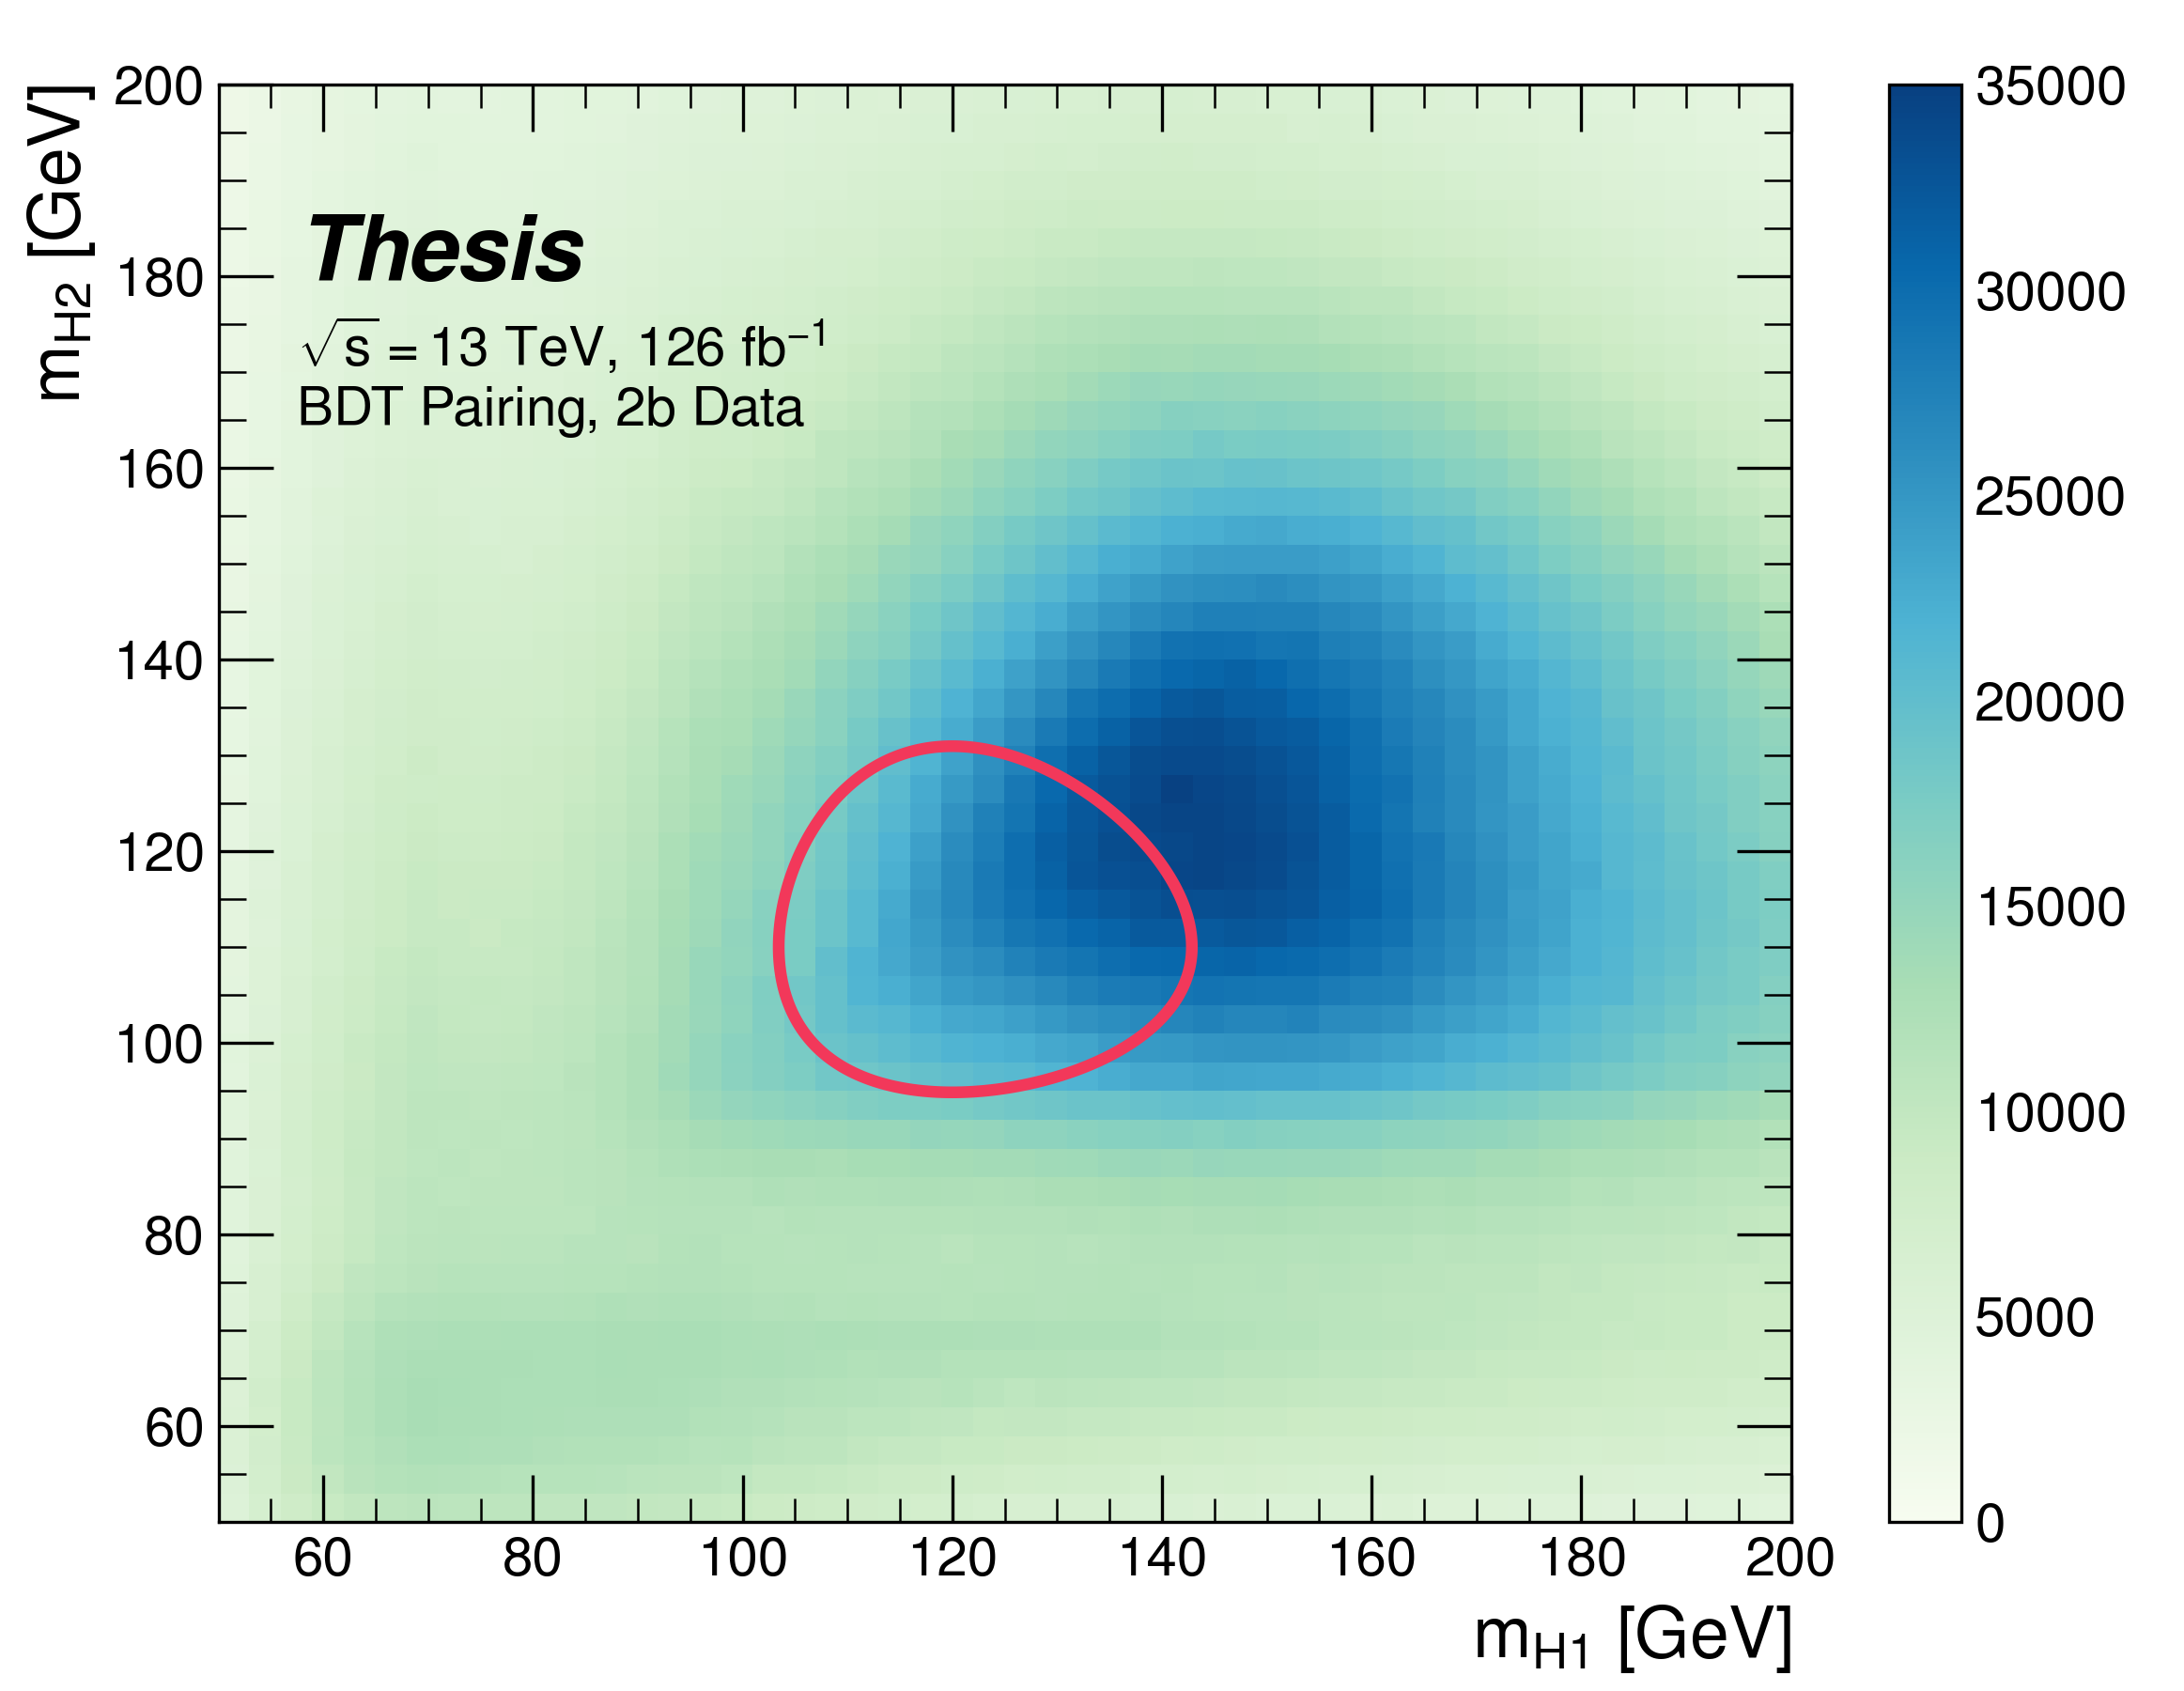
\includegraphics[width=0.48\textwidth]{figures/BDT-pairing-2b-massplane.png}
		 }
\subfloat[$\min\Delta R$ pairing]{\label{fig:mindR-massplane}
		  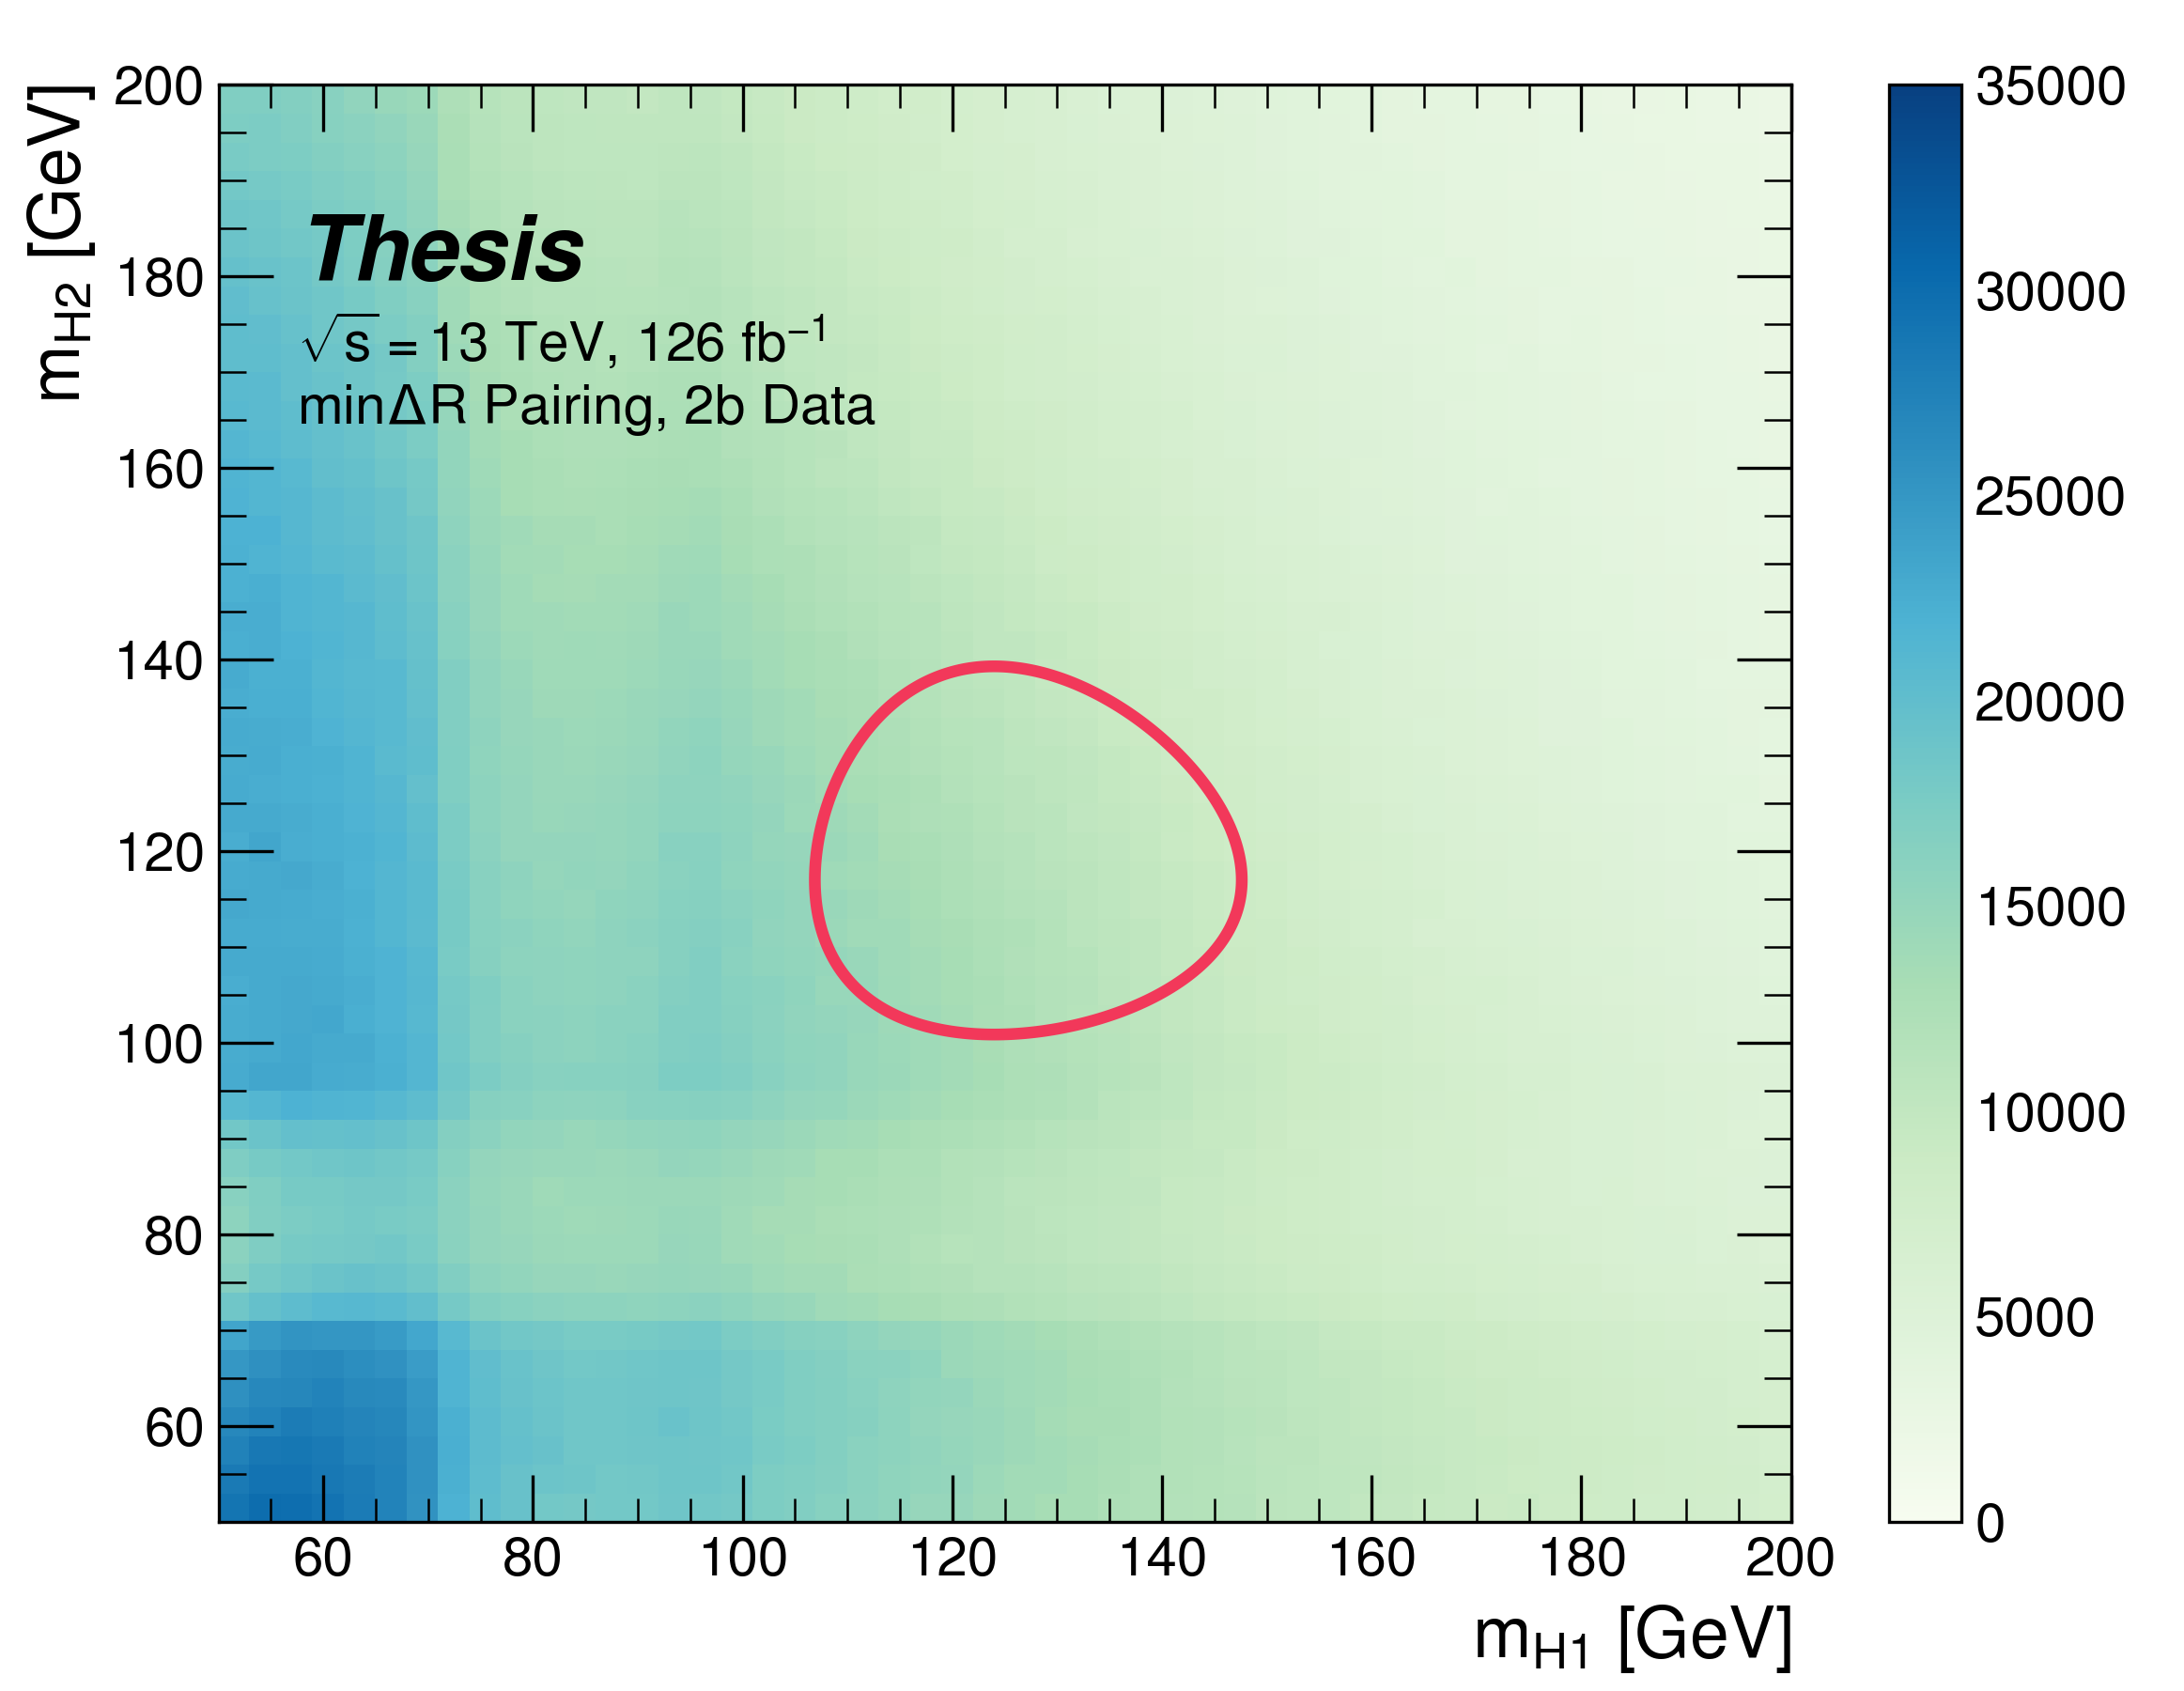
\includegraphics[width=0.48\textwidth]{figures/mindR-pairing-2b-massplane.png}
		 }

\subfloat[$D_{HH}$ pairing]{\label{fig:DHH-massplane}
		  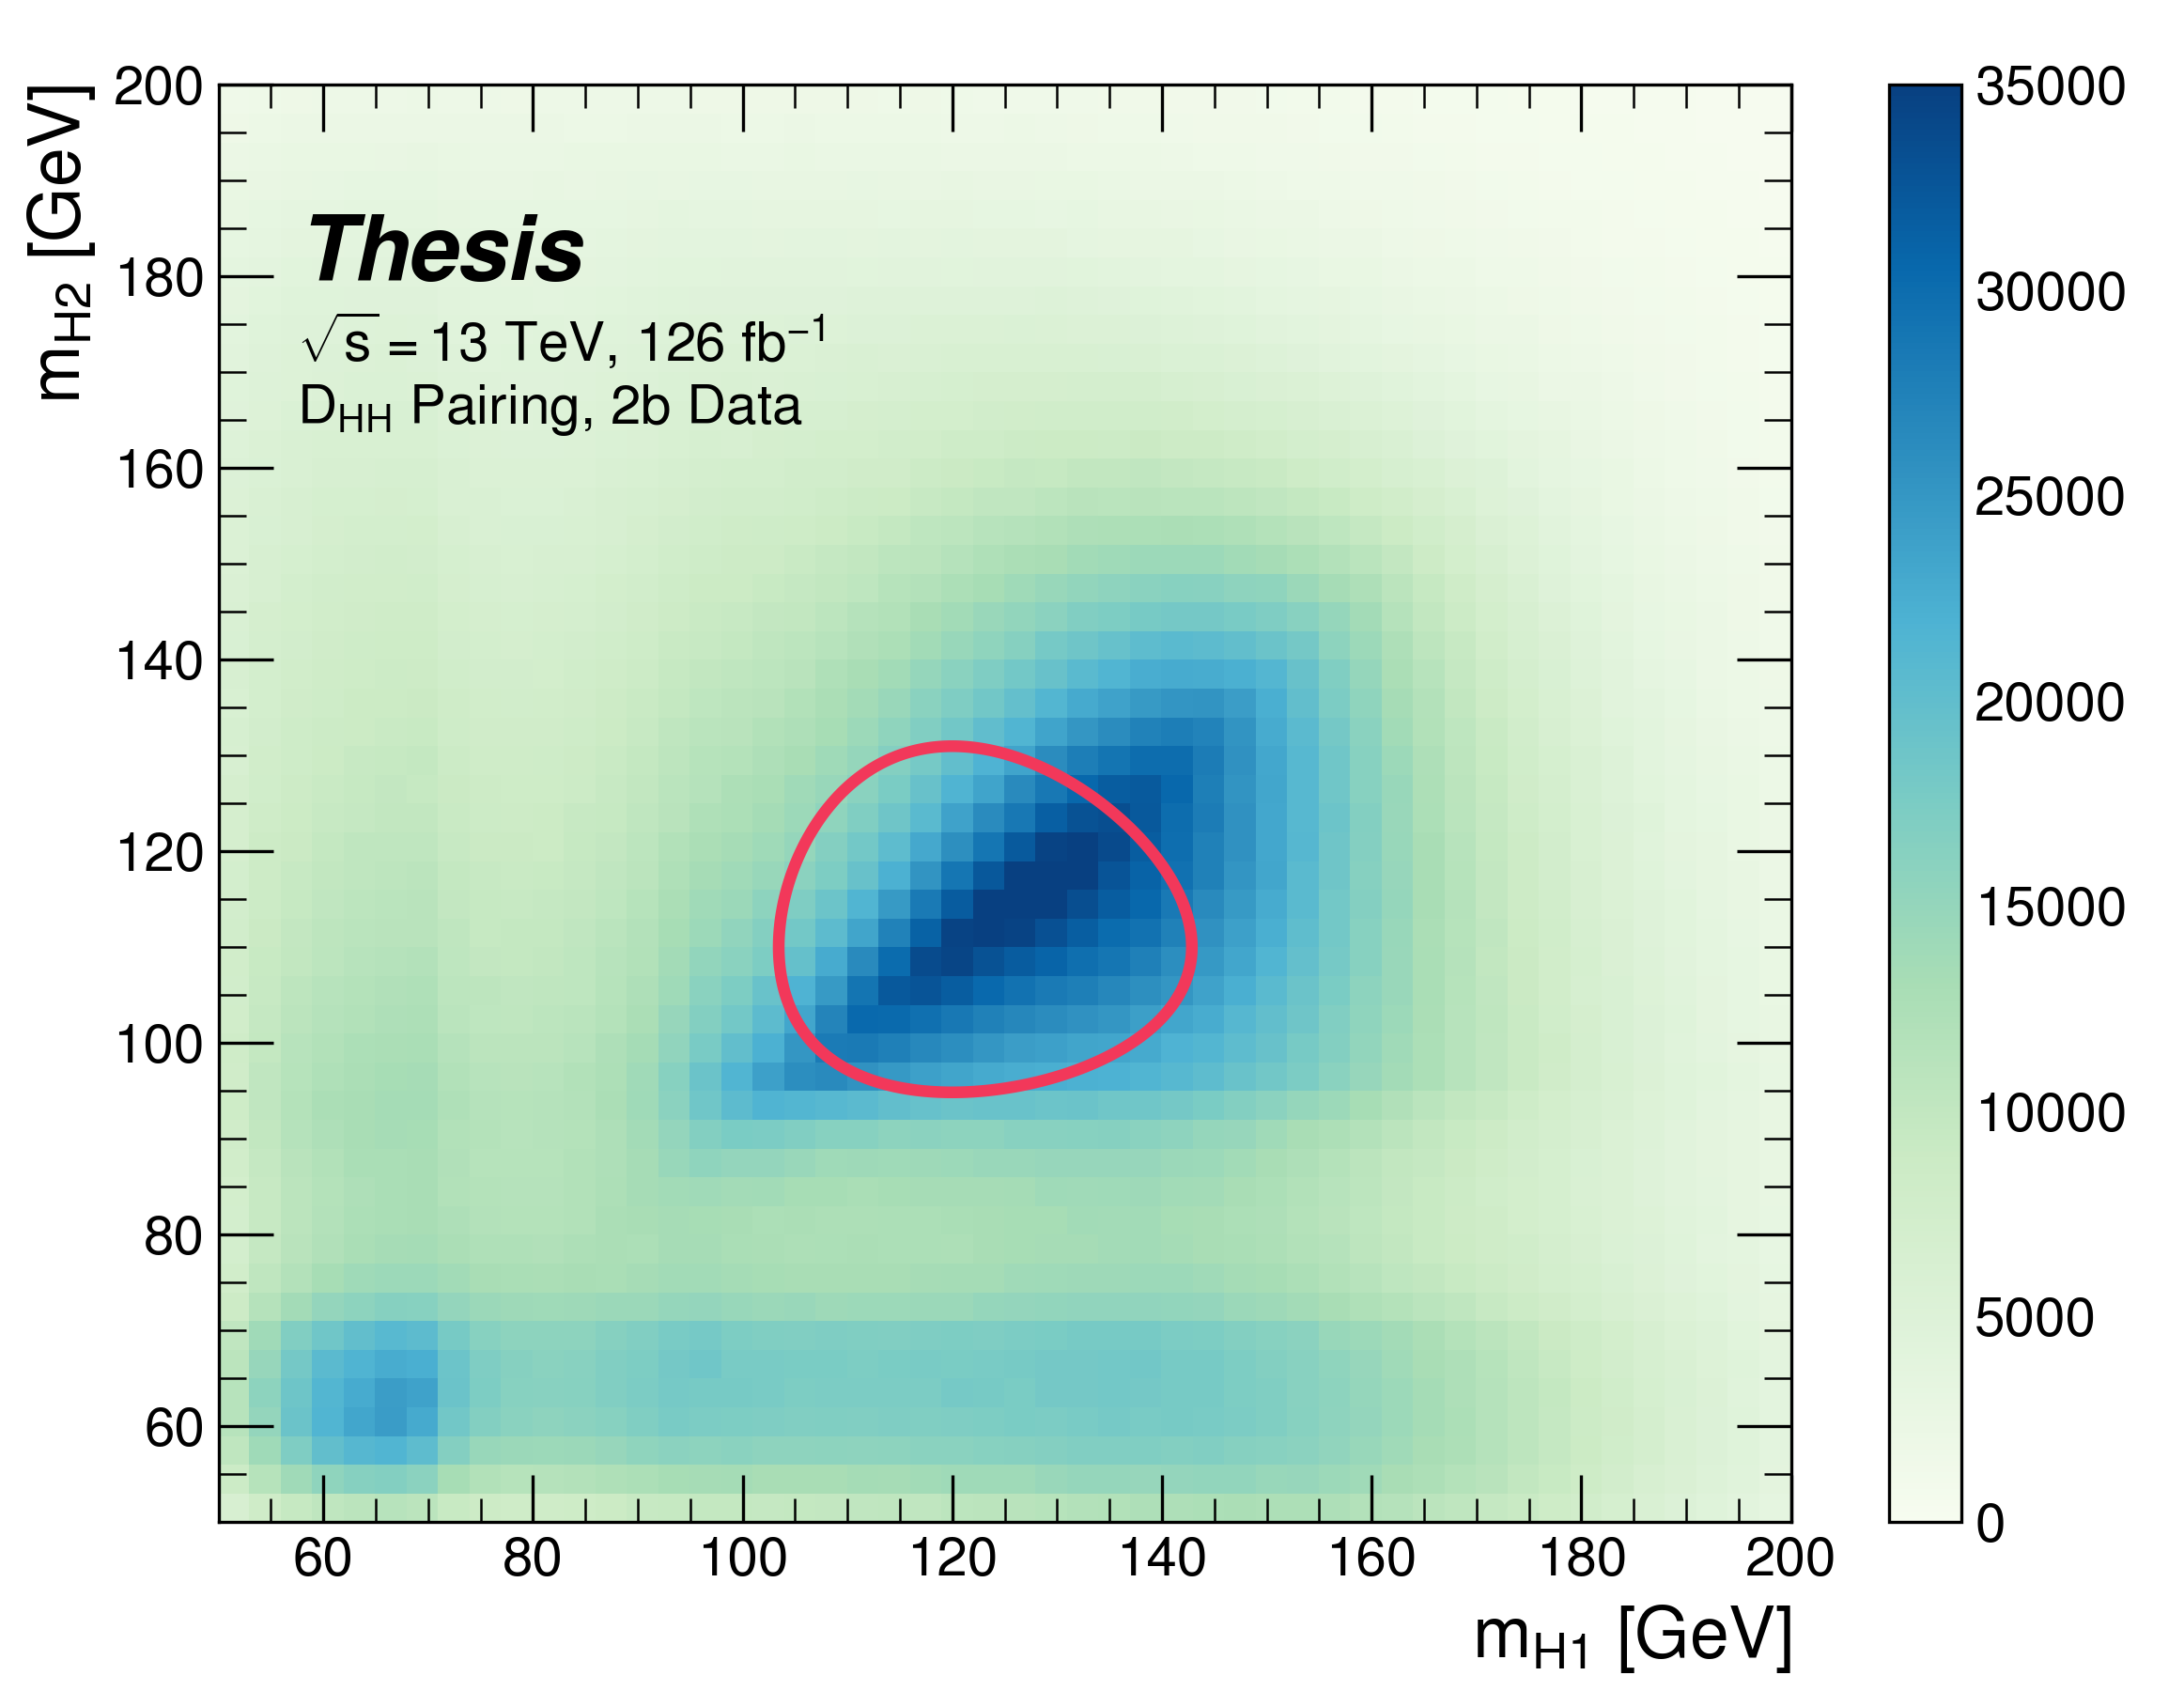
\includegraphics[width=0.48\textwidth]{figures/DHH-pairing-2b-massplane.png}
		 }
\caption{\label{fig:pairing-massplanes} Comparison of $m_{H1}$ vs $m_{H2}$ planes for the full Run 2 $2b$ 
dataset with different pairings. As evidenced, this choice significantly impacts where events 
fall in this plane, and therefore which events fall into the various kinematic regions defined in 
this plane (see Section \ref{sec:kinematic-reg}). The signal regions for the resonant/early Run 2 analysis 
are shown for reference for the BDT and $D_{HH}$ pairings, while the the $\min\Delta R$ signal region shifted 
is shifted slightly up and to the right to match the non-resonant 
selection. Note that the band structure around \SI{80}{\GeV} in both $m_{H1}$ and $m_{H2}$ is introduced 
by the top veto described in Section \ref{sec:kinematic-cuts}.}
\end{figure}


\begin{figure}[ht]

\centering
\subfloat[$\kappa_{\lambda} = 1$ (SM)]{\label{fig:mindR-Dhh-sig-kl1}
		  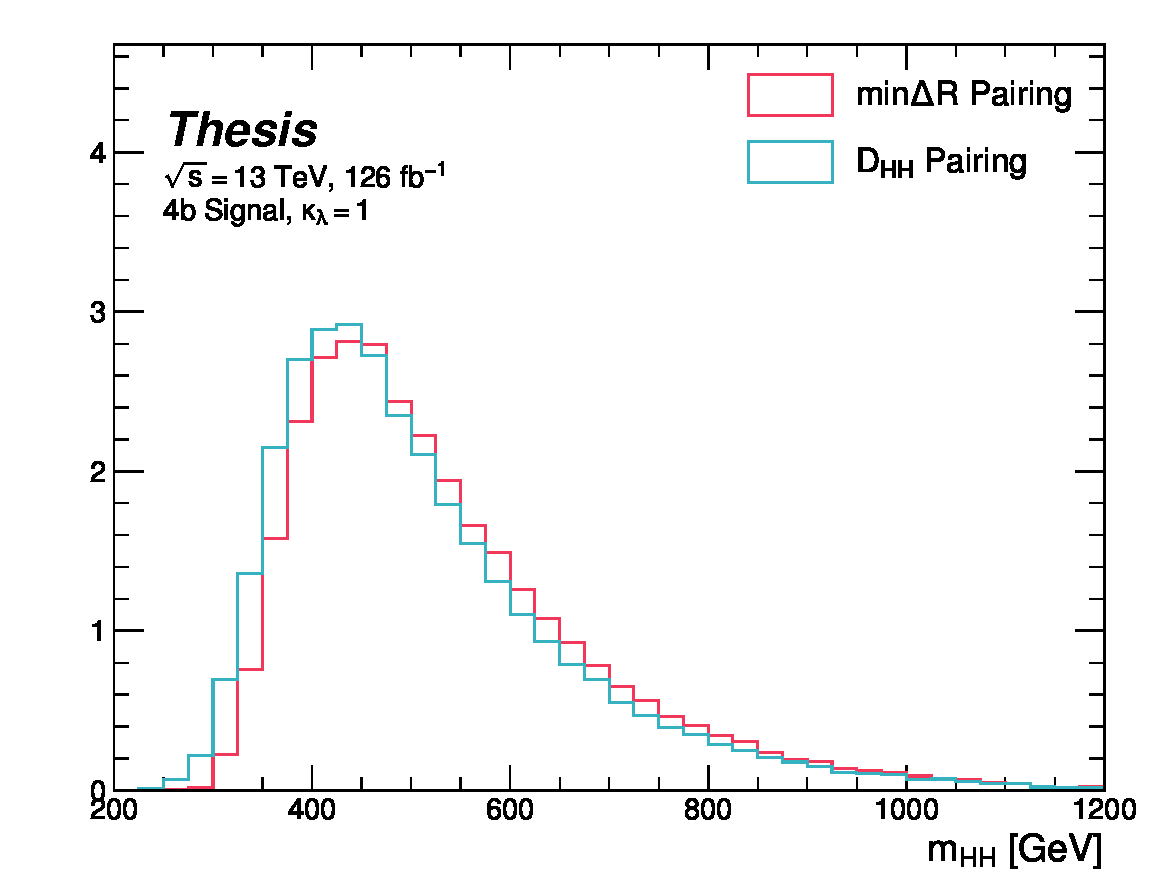
\includegraphics[width=0.48\textwidth]{figures/mindR-vs-Dhh-kl-1.pdf}
		 }
\subfloat[$\kappa_{\lambda} = -10$]{\label{fig:mindR-Dhh-sig-kl--10}
		  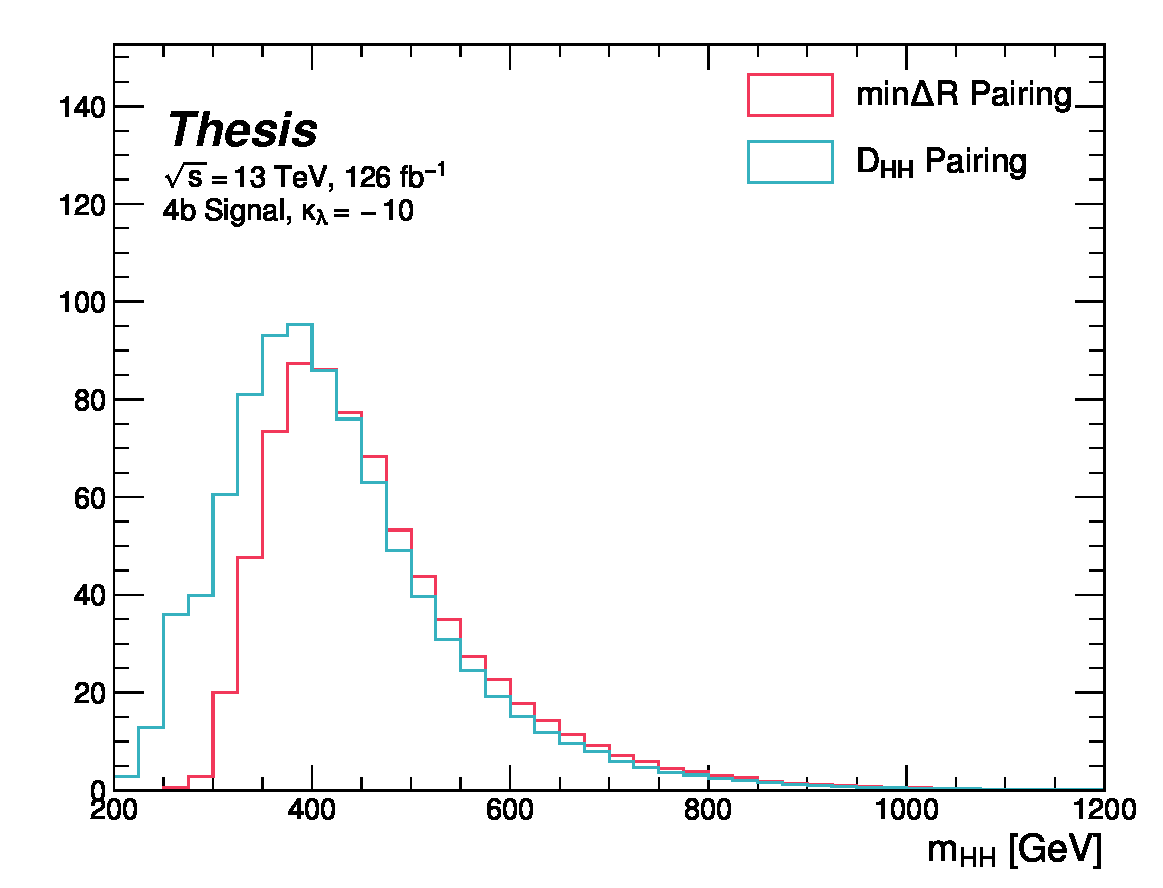
\includegraphics[width=0.48\textwidth]{figures/mindR-vs-Dhh-kl--10.pdf}
		 }

\subfloat[$\kappa_{\lambda} = 3$]{\label{fig:mindR-Dhh-sig-kl-3}
		  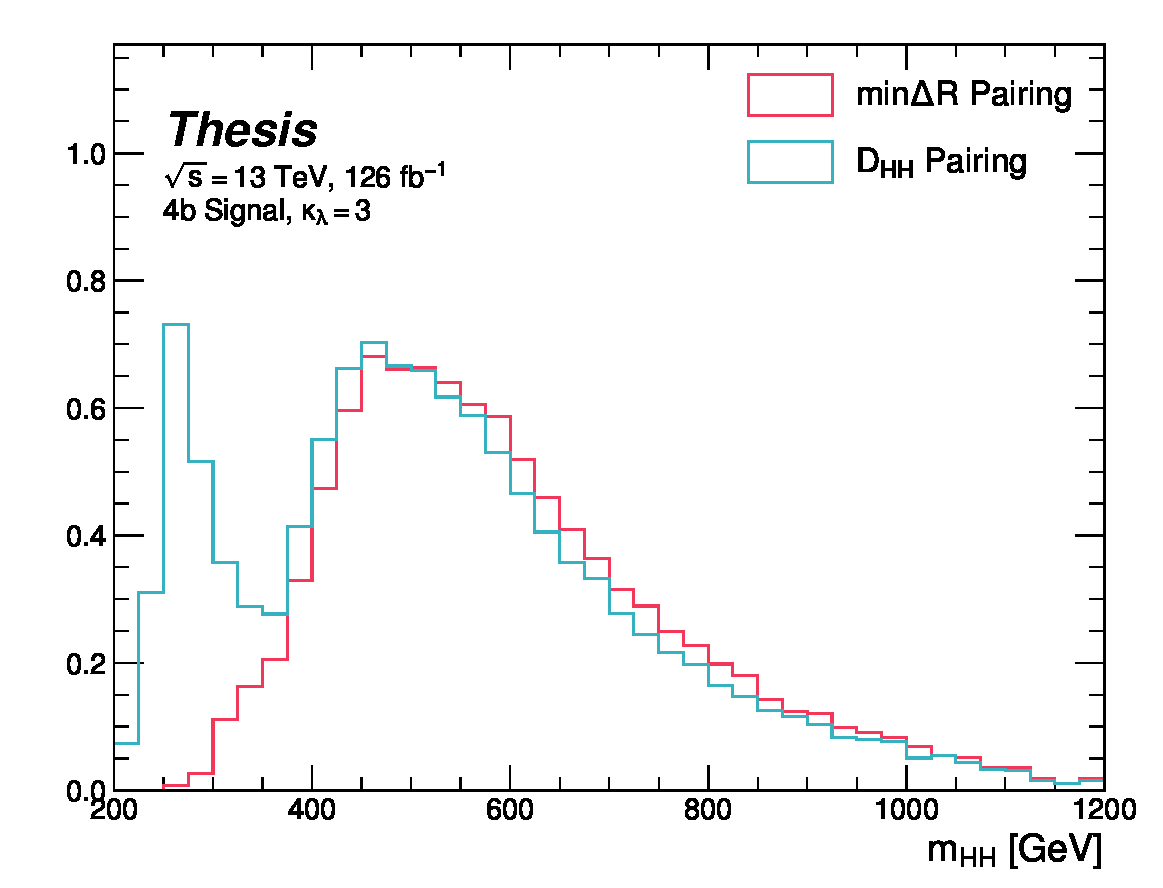
\includegraphics[width=0.48\textwidth]{figures/mindR-vs-Dhh-kl-3.pdf}
		 }
\subfloat[$\kappa_{\lambda} = 10$]{\label{fig:mindR-Dhh-sig-kl-10}
		  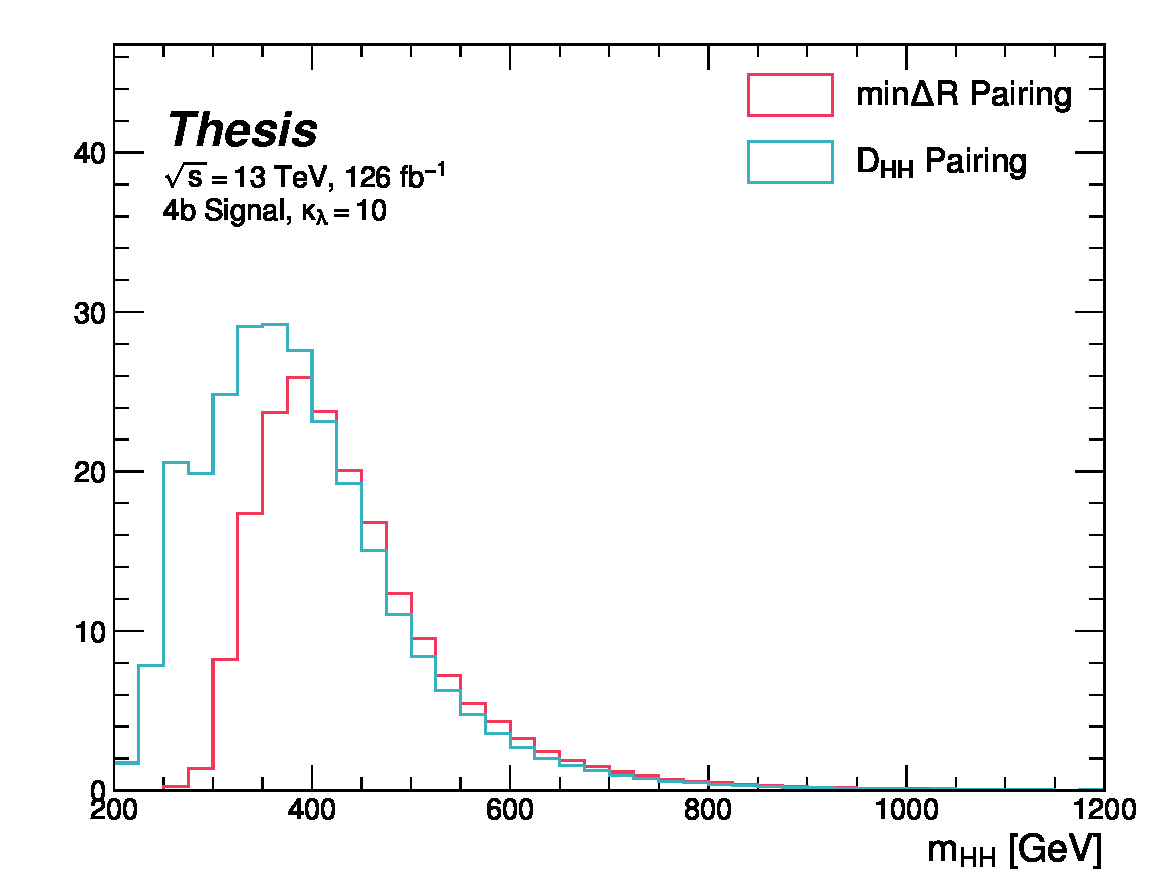
\includegraphics[width=0.48\textwidth]{figures/mindR-vs-Dhh-kl-10.pdf}
		 }
\caption{\label{fig:pairing-signal} 
Comparison of signal distributions in the respective signal regions for the $\min\Delta R$ and 
$D_{HH}$ pairing for various values of the Higgs trilinear coupling in the respective signal regions. The 
distributions are quite similar at the Standard Model point, but for other variations, $\min\Delta R$ does not 
pick up the low mass features.}
\end{figure}


\subsection{Resonant Pairing Strategy}

For the resonant analysis, a Boosted Decision Tree (BDT) is used for the pairing.
The boosted decision tree is given the total separation between the two jets in
each of the two pairs ($\Delta R_{1}$ and $\Delta R_{2}$), the pseudo-rapidity
separation between the two jets in each pair ($\Delta \eta_{1}$ and
$\Delta \eta_{2}$), and the angular separation between the two jets in each pair
in the $x$~--~$y$ plane ($\Delta \phi_{1}$ and $\Delta \phi_{2}$). The total
separations ($\Delta R$s) are provided in addition to the components in order to
avoid requiring the boosted decision tree to reconstruct these variables in
order to use them. For these variables, pair 1 is the pair with the highest
scalar sum of jet \pt{}s, and pair 2 the other pair.

The boosted decision tree is also parameterized on the di-Higgs mass (\mhh)
by providing this as an additional feature. Since the boosted decision tree is
trained on correct and incorrect pairings in signal events, there will be exactly one
correct pairing and two incorrect pairings in the training set for each \mhh
value present in that set. As a result, this variable cannot, in itself,
distinguish a correct pairing from an incorrect pairing, and therefore the
inclusion of this variable simply serves to parameterize the BDT on
\mhh\footnote{That is, the conditions placed on the other variables by the BDT
	vary with \mhh.}.

The boosted decision tree was trained on one quarter of the total AFII
simulated scalar MC statistics, using the Gradient-based One Side Sampling
(GOSS) algorithm which allows rapid training with very large datasets. A
preselection was applied requiring events to have four jets with a \pt of at
least \SI{35}{\GeV}. Note that this is a looser requirement than the
\SI{40}{\GeV} used in the analysis selection, and is meant to increase the
available statistics for events with low \mhh and to ensure a better
performance as a function of that variable. Events were also required to have
four distinct jets that could be geometrically matched (to within
$\Delta R \leq 0.4$) to the \bquarks. The events used to train the BDT were
not included when the analysis was run on these signal simulations. The
boosted decision tree was constructed with the following hyperparameters:\\
\code{min_data_in_leaf=50,\\
	num_leaves=180,\\
	learning_rate=0.01}

These hyperparameters were optimized using a Bayesian optimization
procedure~\cite{skopt}. Three fold cross-validation was used to perform this
optimization without the need for an additional sample, while avoiding
over-training on signal events.

\subsection{Non-resonant Pairing Strategy}
For the non-resonant analysis, a simpler pairing algorithm is used, which 
proceeds as follows: in a given event, Higgs candidates for each possible pairing
are sorted by the $p_{T}$ of the vector sum of constituent jets. The angular separation,
$\dr$ is computed between jets in the each of the leading Higgs candidates, and the 
pairing with the smallest separation ($\dr_{jj}$) is selected. This method will be 
referred to as $\min{\dr}$ in the following.

The primary motivation for the use of this pairing in the non-resonant search is a 
\emph{smooth mass plane}: by efficiently discarding low mass events, $\min{\dr}$ removes 
the background peak present in the resonant search while maintaining good pairing 
efficiency for the Standard Model non-resonant signal. This facilitates a background estimate with 
small kinematic bias -- the region in which the background estimate is derived is 
more similar to the signal region. 

Along with discarding low mass background, there is a corresponding loss of low mass signal.
This predominantly impacts points away from the Standard Model (see Figure \ref{fig:pairing-signal}), 
but, because the $4b$ channel has the strongest contribution near the Standard Model and because of the 
large low mass background present with other pairing methods, the impact on analysis sensitivity 
is mitigated. The $\min{\dr}$ pairing is thus adopted for the non-resonant search.

\FloatBarrier
\clearpage
\section{Background Reduction and Top Veto}
\label{sec:kinematic-cuts}

Choosing a pairing of the four b-tagged jets fully defines the di-Higgs candidate system used for each event in the remainder of the analysis chain. A requirement of
$\abs{\Delta\eta_{\higgs\higgs}} < 1.5$ on this di-Higgs candidate system mitigates
QCD multijet background.

In order to mitigate the hadronic \ttbar background, a top veto is then applied,
removing events consistent with a \HepProcess{\Pqt \to \Pqb (\PW \to \Pq_{1} \Paq_{2})}
decay.

The jets in the event are separated into \emph{HC jets} which are
the four jets used to build the Higgs candidates, and \emph{non-HC jets}, the
other jets (passing the \pt and $\abs{\eta}$ requirements) in the event.

\PW candidates are built by forming all possible pairs of all jets in each event.
With $n$ jets, there are $\binom{n}{2}$ such pairs. \Pqt candidates are then built
by pairing each \PW candidate with each HC jet (for $4\binom{n}{2}$ combinations).
Note that all jets in a \Pqt candidate must be distinct (i.e. a HC jet may not be
used both on its own and in a \PW candidate).

With $m_{\Pqt}$ denoting the invariant mass of the \Pqt candidate, and $m_{\PW}$
the invariant mass of the \PW candidate, the quantity
\begin{equation}
	\label{eqn:xwt-def}
	X_{\PW\Pqt} = \sqrt{\qty(\frac{m_{\PW} - \SI{80.4}{\GeV}}{0.1\cdot m_{\PW}})^{2} + \qty(\frac{m_{\Pqt} - \SI{172.5}{\GeV}}{0.1\cdot m_{\Pqt}})^{2}}
\end{equation}

is constructed for each combination.

Events are then vetoed if the minimum $X_{\PW\Pqt}$ over all combinations is
less than 1.5.

The same definitions and procedures are used for both the resonant and non-resonant analyses.
However, for the non-resonant search, the top candidates considered for $X_{\PW\Pqt}$ have the 
additional requirement that the jet used for the $b$ is $b$-tagged. While this is identical
to the resonant analysis by definition for $4b$ events, it does change the set of events 
considered in lower tag regions, in particular for the $2b$ events considered in the derivation
of the background estimate. Such a change is found to reduce the impact of background systematics
by increasing $2b$ support in the high $X_{\PW\Pqt}$ kinematic region. \todo{Insert plots of variables}

\FloatBarrier
\clearpage
\section{Kinematic Region Definition}
\label{sec:kinematic-reg}
As has been mentioned, an important piece of the analysis is the plane defined by the 
two Higgs candidate masses (the \emph{Higgs candidate mass plane}). After the selection
described above, a signal region is defined by requiring $X_{\higgs\higgs} < 1.6$, where:
\begin{equation}
	\label{eqn:xhh-def}
	X_{\higgs\higgs} = \sqrt{\qty(\frac{\mh1 - c_1}{0.1\cdot\mh1})^{2} + 
	\qty(\frac{\mh2 - c_2}{0.1\cdot\mh2})^{2}}
\end{equation}
with \mh1, \mh2 the leading and subleading Higgs candidate masses, $c_{1}$ and $c_{2}$ correspond
to the center of the signal region, and the denominator provides a Higgs candidate mass 
dependent resolution of 10~\%. For consistency with the $HH$ decay hypothesis, $c_{1}$ and $c_{2}$
are nominally (\SI{125}{\GeV}, \SI{125}{\GeV}). However, these are allowed to vary due to 
energy loss, with specific values chosen described below. The selection of these values is 
one of several significant differences between the regions defined for the resonant and non-resonant search.
We describe both below.

\subsection{Resonant Kinematic Regions}
For the resonant analysis, the signal region is centered at (\SI{120}{\GeV}, \SI{110}{\GeV}) 
to account for energy loss leading to the Higgs masses being under-reconstructed. Note that leading and 
subleading Higgs candidates are defined according to the 
\emph{scalar sum} of constituent jet $p_{T}$.

For the background estimation, two regions are defined which are roughly concentric around the 
signal region: a \emph{validation region} which 
consists of those events not in the signal region, but which do pass
\begin{equation}
	\label{eqn:val-reg-def}
	\sqrt{\qty(\mh1 - 1.03 \times \SI{120}{\GeV})^{2} + \qty(\mh2 - 1.03 \times
		\SI{110}{\GeV})^{2}} < \SI{30}{\GeV}
\end{equation}
and a \emph{control region} which consists of those events not in the signal or validation
regions, but which do pass
\begin{equation}
	\label{eqn:ctrl-reg-def}
	\sqrt{\qty(\mh1 - 1.05 \times \SI{120}{\GeV})^{2} + \qty(\mh2 - 1.05 \times
		\SI{110}{\GeV})^{2}} < \SI{45}{\GeV}
\end{equation}

For simplicity, the SR/VR/CR definitions from the early Run 2 paper~\cite{EXOT-2016-31} were chosen 
for the resonant analysis, and were found to be close to optimal. These regions are shown in Figure 
\ref{fig:res-regions}.

\begin{figure}
\centering
\subfloat{
		  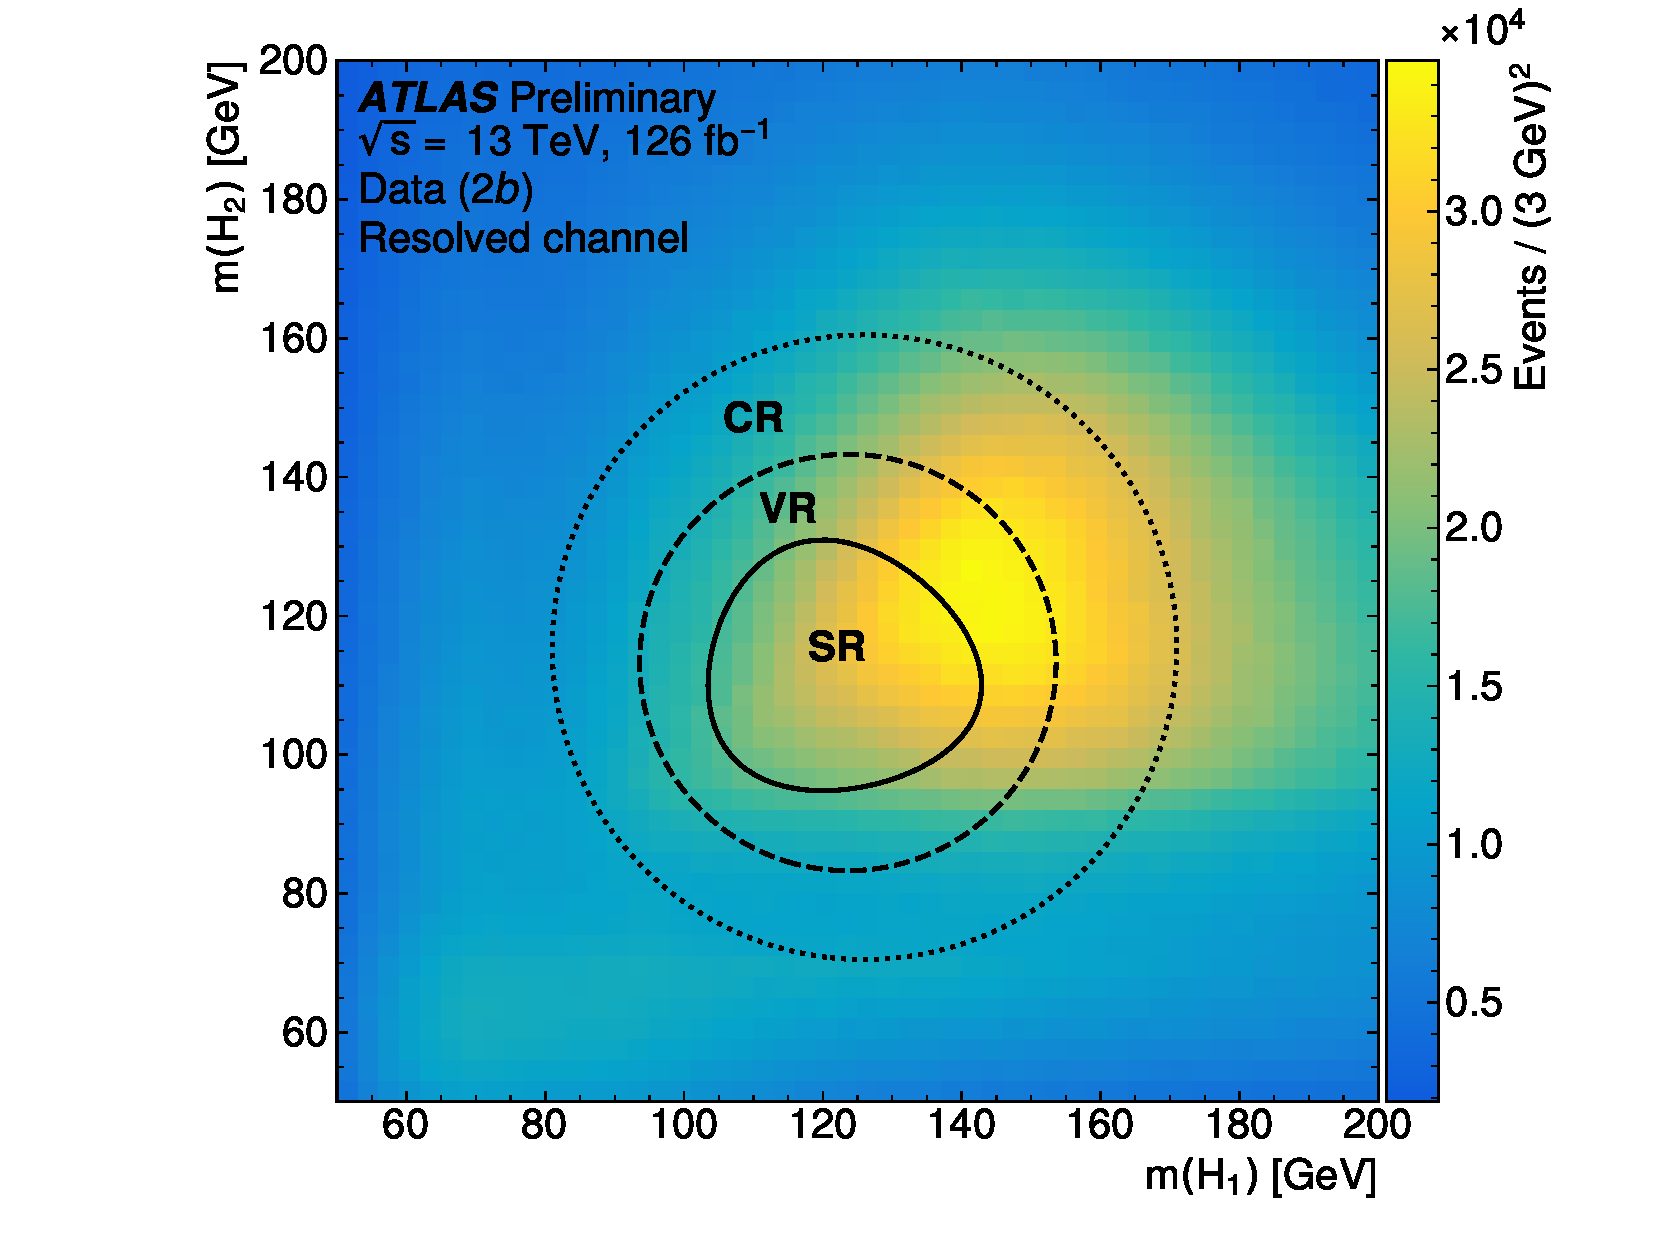
\includegraphics[width=0.8\textwidth]{figures/region-def-resolved.pdf}
  }
\caption{\label{fig:res-regions} Regions used for the resonant search, shown on the $2b$ data  
mass plane. The outermost region (the ``control region'') is used for derivation of the nominal 
background estimate. The innermost region is the signal region, where the signal extraction 
fit is performed. The region in between (the ``validation region'') is used for the assessment of an 
uncertainty.}
\end{figure}

\subsection{Non-resonant Kinematic Regions}
For the non-resonant analysis the signal region is centered at (\SI{124}{\GeV}, \SI{117}{\GeV}),
corresponding to the means of \emph{correctly paired} Standard Model signal events. The shape of 
the signal region (other than this change of center) was found to remain optimal.

For the non-resonant search, leading and subleading Higgs candidates are defined according to the 
\emph{vector sum} of constituent jet $p_{T}$, more closely corresponding to the $1\rightarrow 2$ decay assumption
behind the $\min{\dr}$ pairing algorithm. 

Two areas for improvement were identified in the resonant analysis, which will be discussed in more detail below: 
\emph{signal contamination} of the validation region (which impacts the uncertainty assessed due to extrapolation)
and \emph{large nuisance parameter pulls} for this uncertainty, corresponding to a rough assumption that the 
validation region is closer to the signal region in the mass plane, and so offers a better estimate of the 
signal region. Extensive cross-checks were performed for the resonant search, which demonstrated minimal 
bias due to the signal contamination and healthy behavior of the signal extraction fit, despite 
the large pulls. However, these large pulls imply that the nominal estimate may be improved by 
incorporating some of the information entering the definition of the extrapolation uncertainty. Further, 
the resonant search benefits from a set of highly peaked signals, such that the smooth nature of the 
background helps to mitigate signal contamination bias. With the broad non-resonant signals, 
a bias due to signal contamination becomes more of a concern, such that addressing this is highly 
motivated.

A redesign of the control and validation regions is therefore performed for 
the non-resonant analysis. The outer boundary defined by the shifted resonant control region:
\begin{equation}
	\label{eqn:ctrl-reg-def}
	\sqrt{\qty(\mh1 - 1.05 \times \SI{124}{\GeV})^{2} + \qty(\mh2 - 1.05 \times
		\SI{117}{\GeV})^{2}} < \SI{45}{\GeV}
\end{equation}
is kept, roughly corresponding to combining the regions used for the resonant analysis. In order 
to assess the variation of the background estimate, two sets of regions are desired, so this combined 
region is split into \emph{quadrants}, that is, divided into four pieces along axes that intersect 
with the signal region center. To avoid kinematic bias, quadrants on opposite sides of the signal 
region are paired, with these pairs corresponding to the non-resonant control and validation regions.

The particular orientation of the regions is chosen such that region centers align with the leading
and subleading Higgs candidate masses, corresponding to a set of axes rotated at $45^{\circ}$, with the ``top''
and ``bottom'' quadrants together comprising the control region, and the other set (``left'' and ``right'')
the validation region. These regions are shown in Figure \ref{fig:nonres-regions}
\begin{figure}
\centering
\subfloat{
		  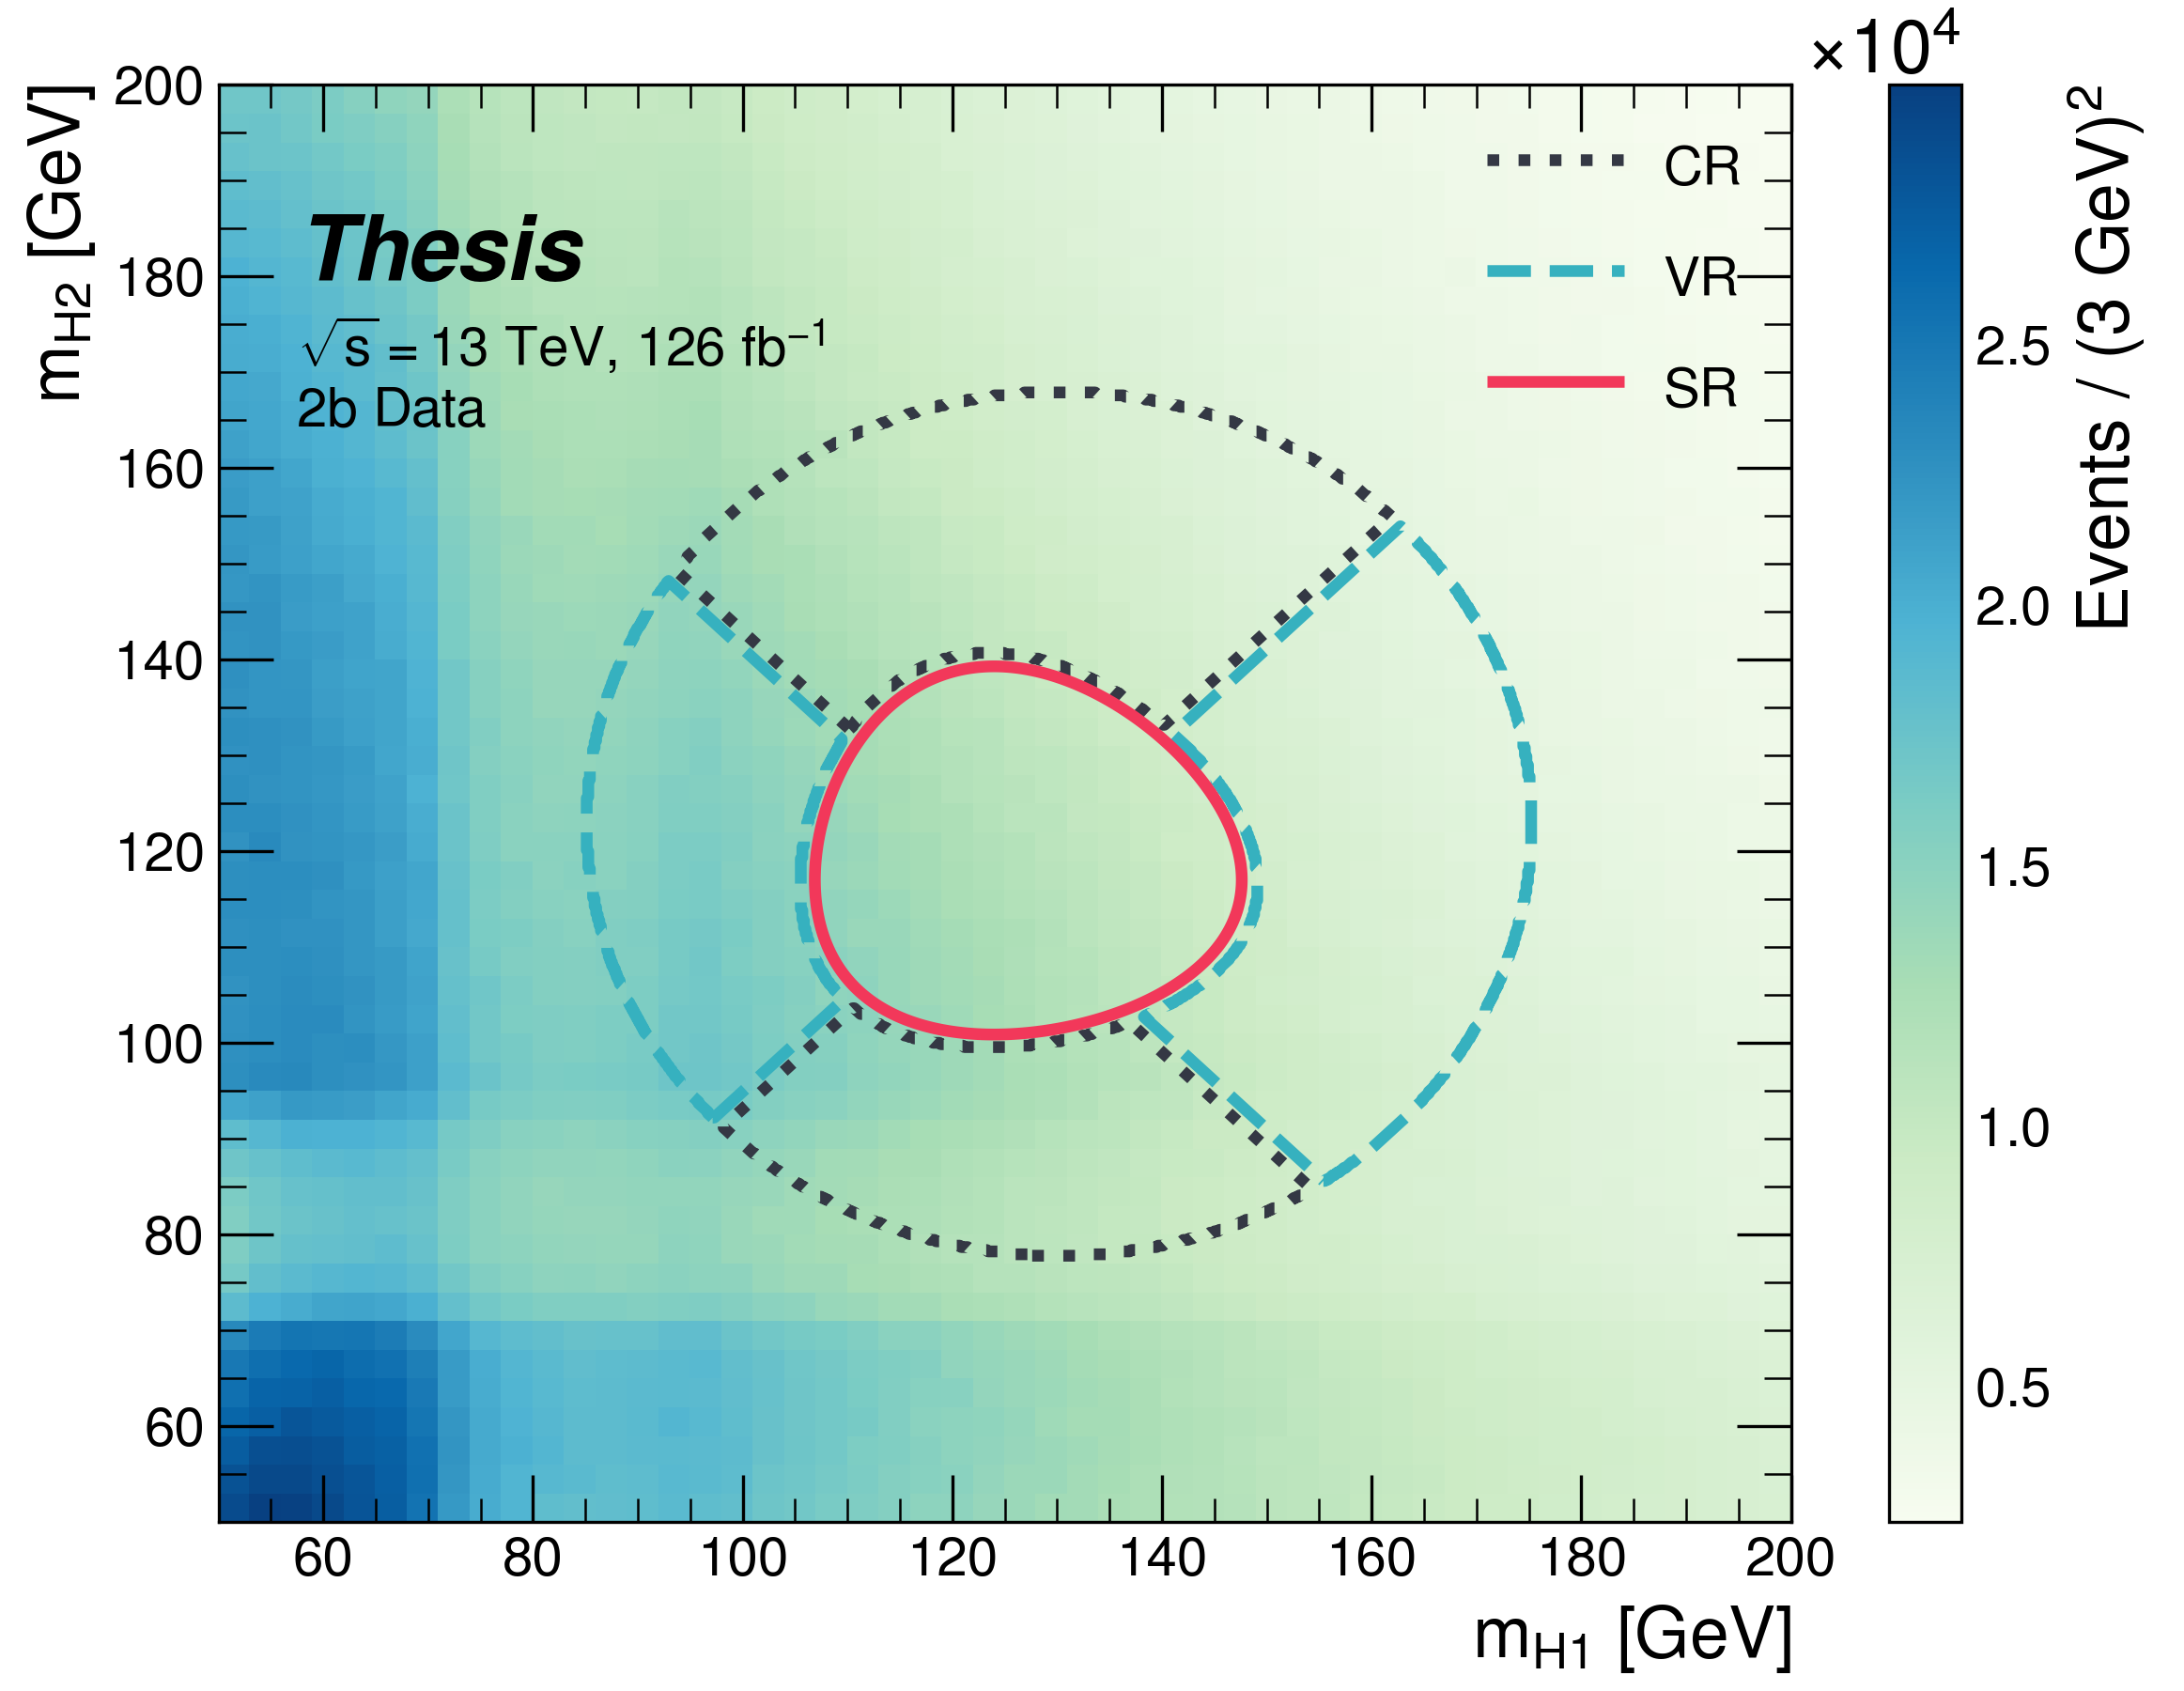
\includegraphics[width=0.8\textwidth]{figures/nonres-regions.png}
  }
\caption{\label{fig:nonres-regions} Regions used for the non-resonant search. The ``top''
and ``bottom'' quadrants together comprise the control region, in which the nominal background 
estimate is derived. The``left'' and ``right'' quadrants together comprise the validation region, 
which is used to assess an uncertainty. The signal region, in the center, is where the signal extraction 
fit is performed.}
\end{figure}

This design of regions includes a set of events closer to the signal region in the mass plane, leveraging
the assumption that these events are more similar to signal region events, while also including events further away
from the signal region, mitigating signal contamination. This region selection is found to have good performance
in alternate validation regions (see Section \ref{sec:bkgd-validation}).

\subsection{Discriminating Variable}
\label{subsec:disc-var}

The discriminant used for the resonant analysis is \emph{corrected $m_{HH}$}. This
variable is calculated by re-scaling the Higgs candidate four vectors such that
each $m_{H} = \SI{125}{\GeV}$. These re-scaled four-vectors are then summed, and
their invariant mass is the corrected $m_{HH}$. These re-scaled four-vectors are
not used for any other purpose. The effect of this correction, which sharpens
the $m_{HH}$ peak and correctly centers it, is shown
in~\Fig{\ref{fig:m-hh-cor-effect}}.
\begin{figure}[ht]
\centering
\subfloat{
		  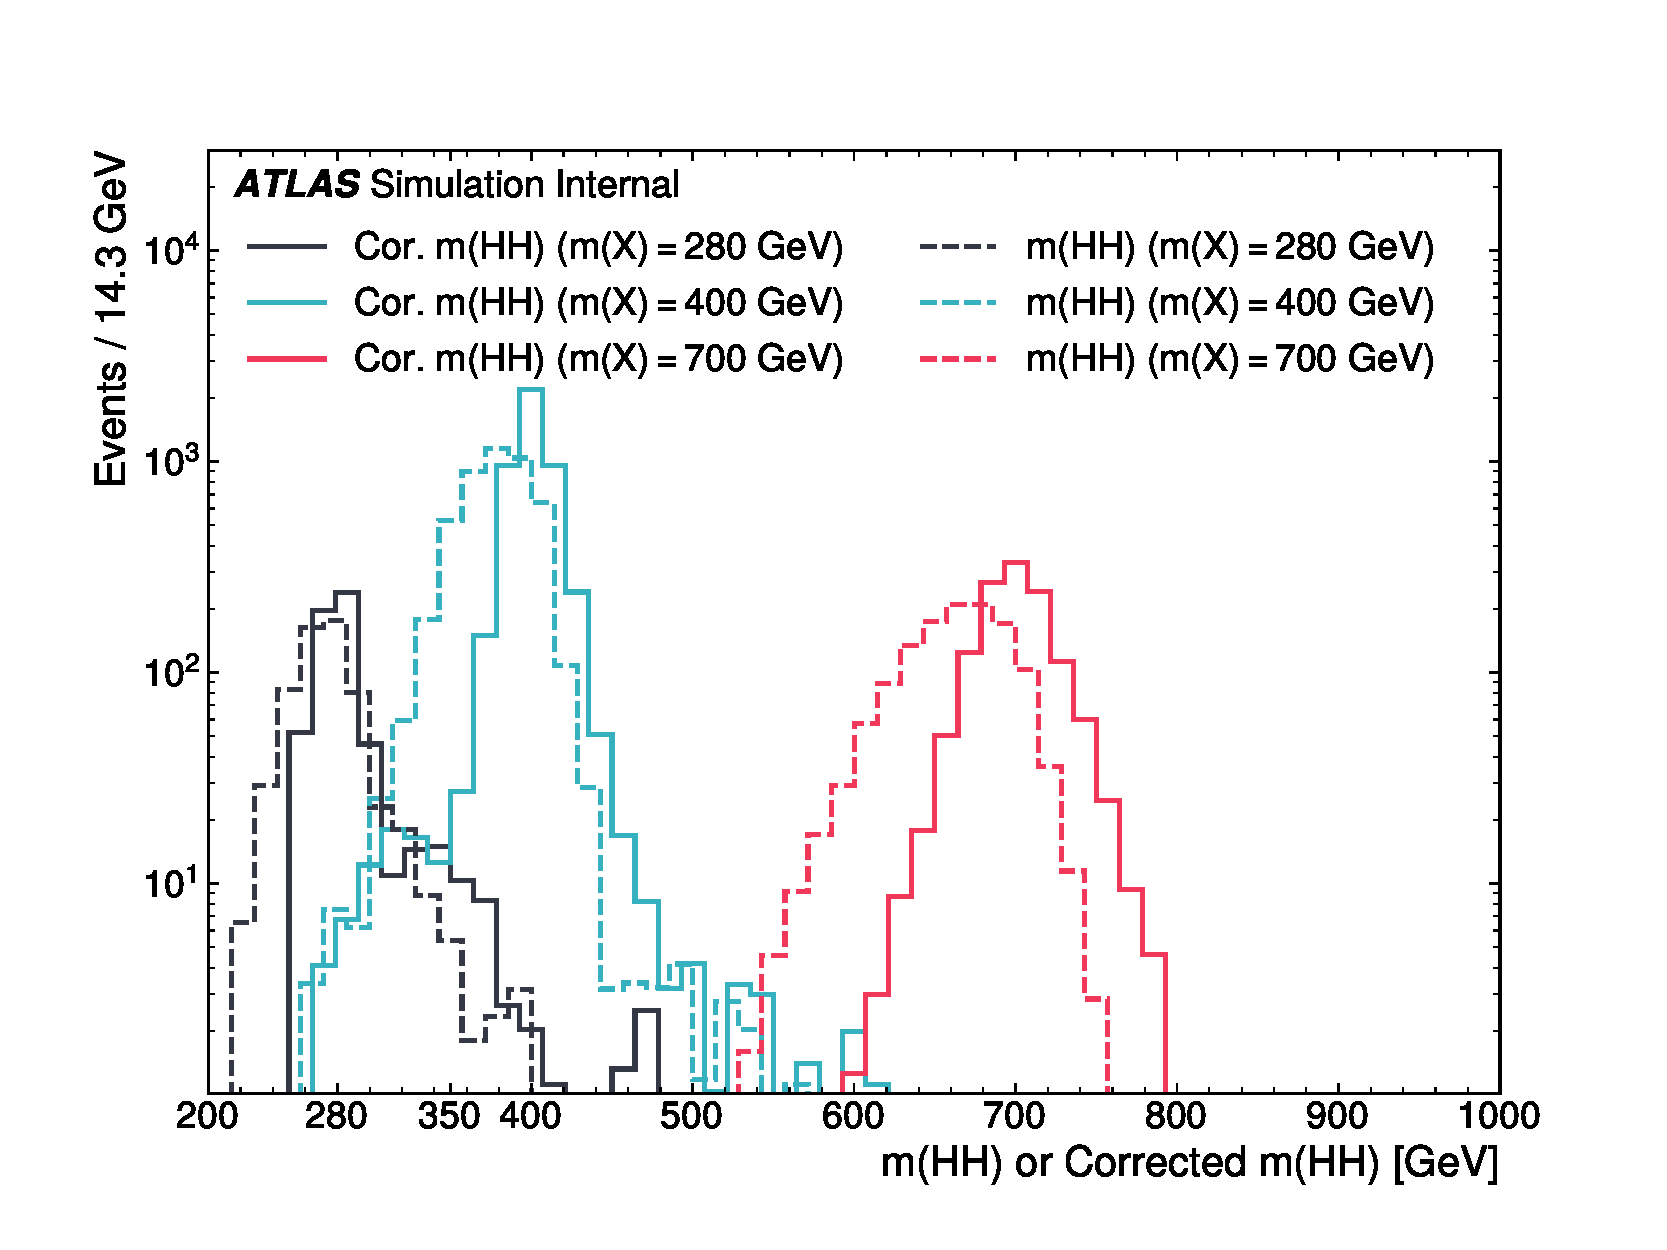
\includegraphics[width=0.8\textwidth]{figures/resolved-m-hh-cor.pdf}
  }
\caption{\label{fig:m-hh-cor-effect} Impact of the $m_{HH}$ correction on a range of spin-0 
resonant signals. The corrected $m_{HH}$ distributions (solid lines) are much sharper and 
more centered on the corresponding resonance masses than the uncorrected $m_{HH}$ distributions 
(dashed).}
\end{figure}

For the non-resonant analysis, due to the broad nature of the signal in \mhh, such a 
correction is not as motivated, and, indeed, is found to have very minimal 
impact. The uncorrected \mhh (just referred to as \mhh) is therefore used 
as a discriminant. To maximize sensitivity, the non-resonant analysis 
additionally uses two variables for categorization: $\Delta \eta_{HH}$, an angular 
variable which, along with \mhh, fully characterizes the $HH$ system~\cite{cosThetastar}, 
and $X_{HH}$, the variable used for the 
signal region definition, which leverages the peaked structure of the 
signal in the ($\mh1$, $\mh2$) plane to split the signal extraction fit into lower and higher
purity regions (highest purity near $X_{HH} = 0$, the center of the signal region).
Distributions of these variables are shown in \todo{plots}. The categorization used for this 
thesis has been optimized to be $2\times 2$ in these variables, with corresponding selections 
$0 \leq \Delta \eta_{HH} \leq 0.75$ and $0.75 \leq \Delta \eta_{HH} \leq 1.5$ for $\Delta \eta_{HH}$, 
and $0 \leq X_{HH} \leq 0.95$ and $0.95 \leq X_{HH} \leq 1.6$ for $X_{HH}$.


\FloatBarrier
\clearpage
\section{Background Estimation}
\label{sec:bkgdestimation}
After the event selection described above, there are
two major backgrounds, QCD and \ttbar. A very similar approach is used 
for both the resonant and the non-resonant analyses, with some small modifications. 
This approach is notably fully data-driven, which is warranted due to 
the flexibility of the estimation method, as well as the high relative proportion of 
QCD background ($>90~\%$), and allows for the use of machine learning methods in the construction of
the background estimate. However, it sacrifices an explicit treatment of the
\ttbar component. Performance of the background estimate on the \ttbar component
is checked explicitly, and minimal impact due to \ttbar 
mis-modeling is seen.

Contributions of single Higgs processes and $\PZ\PZ$ are found 
to be negligible, and the Standard Model $\higgs\higgs$ background
is found to have no impact on the resonant search.

The foundation of the background estimate lies in the derivation of a
reweighting function which matches the kinematics of events with exactly two
\btagged jets to those of events in the higher tagged regions (events with three or four 
\btagged jets). The reweighting function and overall normalization are derived in 
the control region. Systematic bias of this estimate is assessed in the validation 
region. 

For the resonant analysis, the systematic bias is a bias due to extrapolation:
the validation region lies between the control and signal regions. For the 
non-resonant analysis, the bias instead comes from different possible interpolations
of the signal region kinematics -- given the choice of nominal estimate, the validation
region is a conceptually equivalent, but maximally different, signal region estimate.

\subsection{The Two Tag Region}

Events in data with exactly two b-tagged jets are used for the data driven 
background estimate. The hypothesis here is that, due to the presence of 
multiple \btagged jets, the kinematics of such events are similar to the 
kinematics of events in higher b-tagged regions (i.e. events with three and 
four \btagged jets, respectively), and any differences can be corrected by a 
reweighting procedure. The region with three \btagged jets is split into 
two $b$-tagging regions, as described in Section \ref{sec:analysis-selection}, 
with the 3$b$ + 1 loose region used as an additional signal 
region. The lower tagged 3$b$ component (3$b$ + 1 fail) is reserved for validation
of the background modelling procedure. Events with fewer than two \btagged jets are not 
used for this analysis, as they are relatively more different from the higher tag regions.

The nominal event selection requires at least four jets in order to form Higgs
candidates. For the four tag region, these are the four highest $p_{T}$ \btagged 
jets. For the three tag regions, these jets are the three \btagged jets, plus the 
highest $p_{T}$ jet satisfying a loosened $b$-tagging requirement. Similarly, and following 
the approach of the resonant analysis, the two tag region uses the two \btagged jets 
and the two highest $p_{T}$ non-tagged jets to form Higgs candidates. Combinatoric bias 
from selection of different numbers of \btagged jets is corrected as a part of the kinematic 
reweighting procedure through the reweighting of the total number of jets in the event. In this way, 
the full event selection may be run on two tagged events. 

\subsection{Kinematic Reweighting}
The set of two tagged data events is the fundamental piece of the data driven
background estimate. However, kinematic differences from the four tag region
exist and must be corrected in order for this estimate to be useful. Binned 
approaches based on ratios of histograms have been previously considered~\cite{EXOT-2016-31},~\cite{HDBS-2018-18}, 
but are limited in their handling of correlations 
between variables and by the ``curse of dimensionality'', i.e. the dataset
becomes sparser and sparser in ``reweighting space'' as the number of dimensions
in which to reweight increases, limiting the number of variables used for reweighting. 
This leads either to an unstable fit result (overfitting with finely grained bins) or a 
lower quality fit result (underfitting with coarse bins).

Note that even some machine learning methods such as Boosted Decision Trees (BDTs)~\cite{BDT-RW}, may suffer
from this curse of dimensionality, as the depth of each decision tree used is limited by 
the available statistics after each set of corresponding selections (cf. binning in a 
more sophisticated way), limiting the expressivity of the learned reweighting function.

To solve these issues, a neural network based reweighting procedure is used
here. This is a truly multivariate approach, allowing for proper treatment of
variable correlations. It further overcomes the issues associated with binned
approaches by learning the reweighting function directly, allowing for greater
sensitivity to local differences and helping to avoid the curse of
dimensionality.


\subsubsection{Neural Network Reweighting}
Let $p_{4b}(x)$ and $p_{2b}(x)$ be the probability density functions for four and two tag data respectively across 
some input variables $x$. The problem of learning the reweighting function between two and four tag data 
is then the problem of learning a function $w(x)$ such that
\begin{equation}
p_{2b}(x) \cdot w(x) = p_{4b}(x)
\end{equation}
from which it follows that
\begin{equation}
w(x) = \frac{p_{4b}(x)}{p_{2b}(x)}.
\end{equation}

This falls into the domain of density ratio estimation, for which there are a variety
of approaches. The method considered here is modified from ~\cite{NNloss, NNloss1}, and depends on
a loss function of the form
\begin{equation}
\mathcal{L}(R(x)) = \mathbb{E}_{x\sim p_{2b}}[\sqrt{R(x)}]
+\mathbb{E}_{x\sim p_{4b}}[\frac{1}{\sqrt{R(x)}}].
\end{equation}
where $R(x)$ is some estimator dependent on $x$ and $\mathbb{E}_{x\sim p_{2b}}$ and 
$\mathbb{E}_{x\sim p_{4b}}$ are the expectation values with respect to the 2b and 4b probability 
densities. A neural network trained with such a loss function has the objective of finding
the estimator, $R(x)$, that minimizes this loss. It is straightforward to show that
\begin{equation}
\arg \min_{R}\mathcal{L}(R(x)) = \frac{p_{4b}(x)}{p_{2b}(x)}
\end{equation}
which is exactly the form of the desired reweighting function.

In practice, to avoid imposing explicit positivity constraints, the substitution
$Q(x) \equiv \log R(x)$ is made. The loss function then takes the equivalent form
\begin{equation}
\mathcal{L}(Q(x)) = \mathbb{E}_{x\sim p_{2b}}[\sqrt{e^{Q(x)}}]
+\mathbb{E}_{x\sim p_{4b}}[\frac{1}{\sqrt{e^{Q(x)}}}],
\end{equation}
with solution
\begin{equation}
\arg \min_{Q}\mathcal{L}(Q(x)) = \log\frac{p_{4b}(x)}{p_{2b}(x)}.
\end{equation}
Taking the exponent then results in the desired reweighting function.

Note that similar methods for density ratio estimation are available~\cite{NNRW-Nachman},
e.g. from a more standard binary cross-entropy loss. However, these were found to
perform no better than the formulation presented here.

\subsubsection{Variables and Results}
The neural network is trained on a variety of variables sensitive to two vs.
four tag differences. To help bring out these differences, the natural logarithm 
of some of the variables with a large, local change is taken. The 
set of training variables used for the resonant analysis is
\begin{enumerate}
	\item $\log(p_T)$ of the 4th leading Higgs candidate jet
	\item $\log(p_T)$ of the 2nd leading Higgs candidate jet
	\item $\log(\Delta R)$ between the closest two Higgs candidate jets
	\item $\log(\Delta R)$ between the other two Higgs candidate jets
	\item Average absolute value of $\eta$ across the four Higgs candidate jets
	\item $\log(p_T)$ of the di-Higgs system.
	\item $\Delta R$ between the two Higgs candidates
	\item $\Delta \phi$ between the jets in the leading Higgs candidate
	\item $\Delta \phi$ between the jets in the subleading Higgs candidate
	\item $\log(X_{\PW\Pqt})$, where $X_{\PW\Pqt}$ is the variable used for the top veto
	\item Number of jets in the event.
\end{enumerate}
The non-resonant analysis uses an identical set of variables with two notable changes
\begin{enumerate}
	\item The definition of $X_{\PW\Pqt}$ differs from the resonant definition (as described 
	in Section \ref{sec:kinematic-cuts}).
	\item An integer encoding of the two trigger categories is used as an input (variable which 
	takes on the value 0 or 1 corresponding to each of the two categories). This was found to improve
	a mis-modeling near the tradeoff in \mhh of the two buckets.
\end{enumerate}

The neural network used for both resonant and non-resonant reweighting has three 
densely connected hidden layers of 50 nodes each with ReLU activation functions and a single node 
linear output. This configuration demonstrates good performance in the modelling 
of a variety of relevant variables, including \mhh, when compared to a 
range of networks of similar size.

In practice, a given training of the reweighting neural network is subject to variation
due to training statistics and initial conditions. An uncertainty is assigned to account
for this (Section \ref{sec:systematics}), which relies on training an ensemble of
reweighting networks~\cite{DeepEnsembles}. To increase the stability of the background estimate,
the median of the predicted weight for each event is calculated across the ensemble.
This median is then used as the nominal background estimate. This approach is indeed 
seen to be much more stable and to demonstrate a better overall performance than a 
single arbitrary training. Each ensemble used for this analysis consists of 100 
neural networks, trained as described in Section \ref{sec:systematics}.

The training of the ensemble used for the nominal estimate is done in the kinematic
Control Region. The prediction of these networks in the Signal Region is then used
for the nominal background estimate. In addition, a separate ensemble of networks is 
trained in the Validation Region. The difference between the prediction of the nominal 
estimate and the estimate from the VR derived networks in the Signal Region is used to 
assign a systematic uncertainty. Further details on this systematic uncertainty are discussed 
in Section \ref{sec:systematics}.
Note that although the same procedure is used for both Control and Validation Region trained 
networks, only the median estimate from the VR derived reweighting is used for assessing a 
systematic -- no additional ``uncertainty on the uncertainty'' from 
VR ensemble variation is applied.

Each reweighted estimate is normalized such that the reweighted $2b$ yield matches the $4b$ 
yield in the corresponding training region. Note that this applies to each of the networks 
used in each ensemble, where the normalization factor is also subject to the procedure described 
in Section \ref{sec:systematics}. As the median over these normalized weights is not guaranteed 
to preserve this normalization, a further correction is applied such that the $2b$ yield, after 
the median weights are applied, matches the $4b$ yield in the corresponding training region. As no 
preprocessing is applied to correct for the class imbalance between $2b$ and $4b$ events entering 
the training, this ratio of number of $4b$ events ($n(4b)$) over number of $2b$ events ($n(2b)$) is 
folded into the learned weights. Correspondingly, the set of normalization factors described above is 
near $1$ and the learned weights are centered around $n(4b) / n(2b)$ (roughly 0.01 over the full dataset). 
This normalization procedure applies for all instances of the reweighting (e.g. those used for validations 
in Section \ref{sec:bkgd-validation}), with appropriate substitutions of reweighting origin 
(here $2b$) and reweighting target (here $4b$).

Note that, due to different trigger and pileup selections during each year, 
the reweighting is trained on each year separately. An approach of training all of the years 
together with a one-hot encoding was explored, but was found to have minimal 
benefit over the split years approach, and in fact to increase 
the systematic bias of the corresponding background estimate.
Because of this, and because trigger selections for each year significantly impact the kinematics of each year, 
such that categorizing by year is expected to reflect groupings of kinematically similar events and 
to provide a meaningful degree of freedom in the signal extraction fit, the split-year approach is
kept.

The control region closure for the 2018 dataset is shown for the resonant search in Figures \ref{fig:res-Control18-1} 
through \ref{fig:res-Control18-8} and for the non-resonant search in Figures \ref{fig:nonres-Control184b-1} 
through \ref{fig:nonres-Control184b-8} for $4b$ and Figures \ref{fig:nonres-Control183b1l-1} 
through \ref{fig:nonres-Control183b1l-8} for $3b1l$. The impact of this control 
region derived reweighting on the validation region is shown in Figures \ref{fig:res-Validation18-1} 
through \ref{fig:res-Validation18-8} for the resonant search and Figures \ref{fig:nonres-Validation184b-1} 
through \ref{fig:nonres-Validation184b-8} for $4b$ and Figures \ref{fig:nonres-Validation183b1l-1} 
through \ref{fig:nonres-Validation183b1l-8} for $3b1l$ for the non-resonant 
search. 2018 is chosen because it is the largest subset of the data on which the year-by-year reweighting 
is trained. The other years are omitted here for brevity, but demonstrate very similar results. Generally 
good performance is seen, with some occasional mis-modeling. For the resonant 
search, this is most notable in the case of individual jet $p_{T}$. Such mis-modeling may be corrected 
by including the variables in the input set, but this was found to not improve the modeling of $m_{HH}$, 
and so is not done here. This mis-modeling is notable for the non-resonant search in the leading Higgs candidate 
jet $p_{T}$, and is a direct consequence of the trigger category input, which improves modeling of $m_{HH}$.
Results are similar for other years, but are not included here for brevity. 

One other salient feature of the non-resonant plots is the distributions of $m_{H1}$ and $m_{H2}$, which 
emphasize the quadrant region definitions -- the control region has a peak around \SI{125}{\GeV} in $m_{H1}$, 
which may be thought of as ``signal region-like'', motivating this alignment, though consequently the 
distribution of $m_{H2}$ is quite bimodal. The reverse is true for the validation region.

\def\secforfig{background}
\def\figsversion{ggF}
\def\NNTtag{thesis}
\def\weightlabel{bstrap-med}
\def\norwlabel{norw-bstrap-med}
\def\yr{18}

\foreach \region in {Control,Validation}{
	\begin{figure}[ht]
	    \centering
	    \subfloat{\label{fig:res-dRjj1-\region\yr-norw}%
	            \includegraphics[width=0.48\textwidth]{figures/\NNTtag-dRjj-1-\norwlabel-\region-NN-\yr.pdf}
	    }   
	    \subfloat{\label{fig:res-dRjj1-\region\yr}%
	            \includegraphics[width=0.48\textwidth]{figures/\NNTtag-dRjj-1-\weightlabel-\region-NN-\yr.pdf}
	    }   

	    \subfloat{\label{fig:res-dRjj2-\region\yr-norw}%
	            \includegraphics[width=0.48\textwidth]{figures/\NNTtag-dRjj-2-\norwlabel-\region-NN-\yr.pdf}
	    }   
	    \subfloat{\label{fig:res-dRjj2-\region\yr}%
	            \includegraphics[width=0.48\textwidth]{figures/\NNTtag-dRjj-2-\weightlabel-\region-NN-\yr.pdf}
	    }   

	    \subfloat[Before Reweighting]{\label{fig:res-etai-\region\yr-norw}%
	            \includegraphics[width=0.48\textwidth]{figures/\NNTtag-eta-i-\norwlabel-\region-NN-\yr.pdf}
	    }   
	    \subfloat[After Reweighting]{\label{fig:res-etai-\region\yr}%
	            \includegraphics[width=0.48\textwidth]{figures/\NNTtag-eta-i-\weightlabel-\region-NN-\yr.pdf}
	    } 
	    \caption{\textbf{Resonant Search}: Distributions of $\Delta R$ between the closest Higgs Candidate
	      jets, $\Delta R$ between the other two, and average absolute value of HC
	      jet $\eta$ before (left) and after (right) CR derived reweighting for the 20\yr\space \region\space Region.
	      \label{fig:res-\region\yr-1}}
	\end{figure}

	\begin{figure}[ht]
	    \centering
	    \subfloat{\label{fig:res-pT4-\region\yr-norw}%
	            \includegraphics[width=0.48\textwidth]{figures/\NNTtag-pT-4-\norwlabel-\region-NN-\yr.pdf}
	    }   
	    \subfloat{\label{fig:res-pT4-\region\yr}%
	            \includegraphics[width=0.48\textwidth]{figures/\NNTtag-pT-4-\weightlabel-\region-NN-\yr.pdf}
	    }   

	    \subfloat{\label{fig:res-pT2-\region\yr-norw}%
	            \includegraphics[width=0.48\textwidth]{figures/\NNTtag-pT-2-\norwlabel-\region-NN-\yr.pdf}
	    }   
	    \subfloat{\label{fig:res-pT2-\region\yr}%
	            \includegraphics[width=0.48\textwidth]{figures/\NNTtag-pT-2-\weightlabel-\region-NN-\yr.pdf}
	    }   

	    \subfloat[Before Reweighting]{\label{fig:res-pthh-\region\yr-norw}%
	            \includegraphics[width=0.48\textwidth]{figures/\NNTtag-pt-hh-\norwlabel-\region-NN-\yr.pdf}
	    }   
	    \subfloat[After Reweighting]{\label{fig:res-pthh-\region\yr}%
	            \includegraphics[width=0.48\textwidth]{figures/\NNTtag-pt-hh-\weightlabel-\region-NN-\yr.pdf}
	    }
	    \caption{\textbf{Resonant Search}: Distributions of $p_{T}$ of the 2nd and 4th leading Higgs Candidate jets and the $p_{T}$ of the di-Higgs system before (left) and after (right) CR derived reweighting for the 20\yr\space \region\space Region.
	    \label{fig:res-\region\yr-2}}
	\end{figure}

	\begin{figure}[ht]
	    \centering
	    \subfloat[Before Reweighting]{\label{fig:res-njets-\region\yr-norw}%
	            \includegraphics[width=0.48\textwidth]{figures/\NNTtag-njets-\norwlabel-\region-NN-\yr.pdf}
	    }
	    \subfloat[After Reweighting]{\label{fig:res-njets-\region\yr}%
	            \includegraphics[width=0.48\textwidth]{figures/\NNTtag-njets-\weightlabel-\region-NN-\yr.pdf}
	    }
	    \caption{\textbf{Resonant Search}: Distributions of the number of jets before (left) and after (right) CR derived reweighting for the 20\yr\space \region\space Region. A minimum of 4 jets is required in each event in order to form Higgs candidates.
	    \label{fig:res-\region\yr-njet}}
	\end{figure}

	\begin{figure}[ht]
	    \centering
	    \subfloat{\label{fig:res-pT1-\region\yr-norw}%
	            \includegraphics[width=0.48\textwidth]{figures/\NNTtag-pT-1-\norwlabel-\region-NN-\yr.pdf}
	    }   
	    \subfloat{\label{fig:res-pT1-\region\yr}%
	            \includegraphics[width=0.48\textwidth]{figures/\NNTtag-pT-1-\weightlabel-\region-NN-\yr.pdf}
	    }   

	    \subfloat{\label{fig:res-pT3-\region\yr-norw}%
	            \includegraphics[width=0.48\textwidth]{figures/\NNTtag-pT-3-\norwlabel-\region-NN-\yr.pdf}
	    }   
	    \subfloat{\label{fig:res-pT3-\region\yr}%
	            \includegraphics[width=0.48\textwidth]{figures/\NNTtag-pT-3-\weightlabel-\region-NN-\yr.pdf}
	    }   

	    \subfloat[Before Reweighting]{\label{fig:res-dRhh-\region\yr-norw}%
	            \includegraphics[width=0.48\textwidth]{figures/\NNTtag-dR-hh-\norwlabel-\region-NN-\yr.pdf}
	    }   
	    \subfloat[After Reweighting]{\label{fig:res-dRhh-\region\yr}%
	            \includegraphics[width=0.48\textwidth]{figures/\NNTtag-dR-hh-\weightlabel-\region-NN-\yr.pdf}
	    }
	    \caption{\textbf{Resonant Search}: Distributions of $p_{T}$ of the 1st and 3rd leading Higgs Candidate jets and $\Delta R$ between Higgs candidates before (left) and after (right) CR derived reweighting for the 20\yr\space \region\space Region.
	    \label{fig:res-\region\yr-3}}
	\end{figure}

	\begin{figure}[ht]
	    \centering
	    \subfloat{\label{fig:res-eta1-\region\yr-norw}%
	            \includegraphics[width=0.48\textwidth]{figures/\NNTtag-eta-1-\norwlabel-\region-NN-\yr.pdf}
	    }   
	    \subfloat{\label{fig:res-eta1-\region\yr}%
	            \includegraphics[width=0.48\textwidth]{figures/\NNTtag-eta-1-\weightlabel-\region-NN-\yr.pdf}
	    }   

	    \subfloat{\label{fig:res-eta2-\region\yr-norw}%
	            \includegraphics[width=0.48\textwidth]{figures/\NNTtag-eta-2-\norwlabel-\region-NN-\yr.pdf}
	    }   
	    \subfloat{\label{fig:res-eta2-\region\yr}%
	            \includegraphics[width=0.48\textwidth]{figures/\NNTtag-eta-2-\weightlabel-\region-NN-\yr.pdf}
	    }   

	    \subfloat[Before Reweighting]{\label{fig:res-eta3-\region\yr-norw}%
	            \includegraphics[width=0.48\textwidth]{figures/\NNTtag-eta-3-\norwlabel-\region-NN-\yr.pdf}
	    }   
	    \subfloat[After Reweighting]{\label{fig:res-eta3-\region\yr}%
	            \includegraphics[width=0.48\textwidth]{figures/\NNTtag-eta-3-\weightlabel-\region-NN-\yr.pdf}
	    }
	    \caption{\textbf{Resonant Search}: Distributions of $\eta$ of the 1st, 2nd, and 3rd leading Higgs Candidate jets before (left) and after (right) CR derived reweighting for the 20\yr\space \region\space Region.
	    \label{fig:res-\region\yr-4}}
	\end{figure}

	\begin{figure}[ht]
	    \centering
	    \subfloat{\label{fig:res-eta4-\region\yr-norw}%
	            \includegraphics[width=0.48\textwidth]{figures/\NNTtag-eta-4-\norwlabel-\region-NN-\yr.pdf}
	    }   
	    \subfloat{\label{fig:res-eta4-\region\yr}%
	            \includegraphics[width=0.48\textwidth]{figures/\NNTtag-eta-4-\weightlabel-\region-NN-\yr.pdf}
	    }   

	    \subfloat{\label{fig:res-pTh1-\region\yr-norw}%
	            \includegraphics[width=0.48\textwidth]{figures/\NNTtag-pT-h1-\norwlabel-\region-NN-\yr.pdf}
	    }   
	    \subfloat{\label{fig:res-pTh1-\region\yr}%
	            \includegraphics[width=0.48\textwidth]{figures/\NNTtag-pT-h1-\weightlabel-\region-NN-\yr.pdf}
	    }   

	    \subfloat[Before Reweighting]{\label{fig:res-pTh2-\region\yr-norw}%
	            \includegraphics[width=0.48\textwidth]{figures/\NNTtag-pT-h2-\norwlabel-\region-NN-\yr.pdf}
	    }   
	    \subfloat[After Reweighting]{\label{fig:res-pTh2-\region\yr}%
	            \includegraphics[width=0.48\textwidth]{figures/\NNTtag-pT-h2-\weightlabel-\region-NN-\yr.pdf}
	    }
	    \caption{\textbf{Resonant Search}: Distributions of $\eta$ of the 4th leading Higgs Candidate jet and the $p_{T}$ of the leading and subleading Higgs candidates before (left) and after (right) CR derived reweighting for the 20\yr\space \region\space Region.
	    \label{fig:res-\region\yr-5}}
	\end{figure}

	\begin{figure}[ht]
	    \centering
	    \subfloat{\label{fig:res-mh1-\region\yr-norw}%
	            \includegraphics[width=0.48\textwidth]{figures/\NNTtag-m-h1-\norwlabel-\region-NN-\yr.pdf}
	    }   
	    \subfloat{\label{fig:res-mh1-\region\yr}%
	            \includegraphics[width=0.48\textwidth]{figures/\NNTtag-m-h1-\weightlabel-\region-NN-\yr.pdf}
	    }   

	    \subfloat{\label{fig:res-mh2-\region\yr-norw}%
	            \includegraphics[width=0.48\textwidth]{figures/\NNTtag-m-h2-\norwlabel-\region-NN-\yr.pdf}
	    }   
	    \subfloat{\label{fig:res-mh2-\region\yr}%
	            \includegraphics[width=0.48\textwidth]{figures/\NNTtag-m-h2-\weightlabel-\region-NN-\yr.pdf}
	    }   

	    \subfloat[Before Reweighting]{\label{fig:res-mhh-\region\yr-norw}%
	            \includegraphics[width=0.48\textwidth]{figures/\NNTtag-m-hh-\norwlabel-\region-NN-\yr.pdf}
	    }   
	    \subfloat[After Reweighting]{\label{fig:res-mhh-\region\yr}%
	            \includegraphics[width=0.48\textwidth]{figures/\NNTtag-m-hh-\weightlabel-\region-NN-\yr.pdf}
	    }
	    \caption{\textbf{Resonant Search}: Distributions of mass of the leading and subleading Higgs candidates and of the di-Higgs system before (left) and after (right) CR derived reweighting for the 20\yr\space \region\space Region.
	    \label{fig:res-\region\yr-6}}
	\end{figure}

	\begin{figure}[ht]
	    \centering
	   
	    \subfloat{\label{fig:res-dPhi-h1-\region\yr-norw}%
	            \includegraphics[width=0.48\textwidth]{figures/\NNTtag-dPhi-h1-\norwlabel-\region-NN-\yr.pdf}
	    }   
	    \subfloat{\label{fig:res-dPhi-h1-\region\yr}%
	            \includegraphics[width=0.48\textwidth]{figures/\NNTtag-dPhi-h1-\weightlabel-\region-NN-\yr.pdf}
	    }   

	    \subfloat[Before Reweighting]{\label{fig:res-dPhi-h2-\region\yr-norw}%
	            \includegraphics[width=0.48\textwidth]{figures/\NNTtag-dPhi-h2-\norwlabel-\region-NN-\yr.pdf}
	    }   
	    \subfloat[After Reweighting]{\label{fig:res-dPhi-h2-\region\yr}%
	            \includegraphics[width=0.48\textwidth]{figures/\NNTtag-dPhi-h2-\weightlabel-\region-NN-\yr.pdf}
	    }
	    \caption{\textbf{Resonant Search}: Distributions of $\Delta \phi$ between jets in the leading and subleading Higgs candidates before (left) and after (right) CR derived reweighting for the 20\yr\space \region\space Region.
	    \label{fig:res-\region\yr-7}}
	\end{figure}

	\begin{figure}[ht]
	    \centering
	    \subfloat[Before Reweighting]{\label{fig:res-Xwt-\region\yr-norw}%
	            \includegraphics[width=0.48\textwidth]{figures/\NNTtag-X-wt-\norwlabel-\region-NN-\yr.pdf}
	    }
	    \subfloat[After Reweighting]{\label{fig:res-Xwt-\region\yr}%
	            \includegraphics[width=0.48\textwidth]{figures/\NNTtag-X-wt-\weightlabel-\region-NN-\yr.pdf}
	    }
	    \caption{\textbf{Resonant Search}: Distributions of the top veto variable, $X_{\PW\Pqt}$, before (left) and after (right) CR derived reweighting for the 20\yr\space \region\space Region. Reweighting is done after the cut on this variable is applied
	    \label{fig:res-\region\yr-8}}
	\end{figure}
}

\def\NNTtag{thesis}
\def\weightlabel{NN}
\def\norwlabel{no-rw}
\def\yr{18}

\foreach \breg in {4b, 3b1l}
	\foreach \region in {Control,Validation}{
		\begin{figure}[ht]
		    \centering
		    \subfloat{\label{fig:nonres-dRjj1-\region\yr\breg-norw}%
		            \includegraphics[width=0.48\textwidth]{figures/\NNTtag-dRjj-1-\region-\norwlabel-\yr-\breg inclusive.pdf}
		    }   
		    \subfloat{\label{fig:nonres-dRjj1-\region\yr\breg}%
		            \includegraphics[width=0.48\textwidth]{figures/\NNTtag-dRjj-1-\region-\weightlabel-\yr-\breg inclusive.pdf}
		    }   

		    \subfloat{\label{fig:nonres-dRjj2-\region\yr\breg-norw}%
		            \includegraphics[width=0.48\textwidth]{figures/\NNTtag-dRjj-2-\region-\norwlabel-\yr-\breg inclusive.pdf}
		    }   
		    \subfloat{\label{fig:nonres-dRjj2-\region\yr\breg}%
		            \includegraphics[width=0.48\textwidth]{figures/\NNTtag-dRjj-2-\region-\weightlabel-\yr-\breg inclusive.pdf}
		    }   

		    \subfloat[Before Reweighting]{\label{fig:nonres-etai-\region\yr\breg-norw}%
		            \includegraphics[width=0.48\textwidth]{figures/\NNTtag-eta-i-\region-\norwlabel-\yr-\breg inclusive.pdf}
		    }   
		    \subfloat[After Reweighting]{\label{fig:nonres-etai-\region\yr\breg}%
		            \includegraphics[width=0.48\textwidth]{figures/\NNTtag-eta-i-\region-\weightlabel-\yr-\breg inclusive.pdf}
		    } 
		    \caption{\textbf{Non-resonant Search (\breg)}: Distributions of $\Delta R$ between the closest Higgs Candidate
		      jets, $\Delta R$ between the other two, and average absolute value of HC
		      jet $\eta$ before (left) and after (right) CR derived reweighting for the 20\yr\space \breg\space \region\space Region.
		    \label{fig:nonres-\region\yr\breg-1}}
		\end{figure}

		\begin{figure}[ht]
		    \centering
		    \subfloat{\label{fig:nonres-pT4-\region\yr\breg-norw}%
		            \includegraphics[width=0.48\textwidth]{figures/\NNTtag-pT-4-\region-\norwlabel-\yr-\breg inclusive.pdf}
		    }   
		    \subfloat{\label{fig:nonres-pT4-\region\yr\breg}%
		            \includegraphics[width=0.48\textwidth]{figures/\NNTtag-pT-4-\region-\weightlabel-\yr-\breg inclusive.pdf}
		    }   

		    \subfloat{\label{fig:nonres-pT2-\region\yr\breg-norw}%
		            \includegraphics[width=0.48\textwidth]{figures/\NNTtag-pT-2-\region-\norwlabel-\yr-\breg inclusive.pdf}
		    }   
		    \subfloat{\label{fig:nonres-pT2-\region\yr\breg}%
		            \includegraphics[width=0.48\textwidth]{figures/\NNTtag-pT-2-\region-\weightlabel-\yr-\breg inclusive.pdf}
		    }   

		    \subfloat[Before Reweighting]{\label{fig:nonres-pthh-\region\yr\breg-norw}%
		            \includegraphics[width=0.48\textwidth]{figures/\NNTtag-pt-hh-\region-\norwlabel-\yr-\breg inclusive.pdf}
		    }   
		    \subfloat[After Reweighting]{\label{fig:nonres-pthh-\region\yr\breg}%
		            \includegraphics[width=0.48\textwidth]{figures/\NNTtag-pt-hh-\region-\weightlabel-\yr-\breg inclusive.pdf}
		    }
		    \caption{\textbf{Non-resonant Search (\breg)}: Distributions of $p_{T}$ of the 2nd and 4th leading Higgs Candidate jets and the $p_{T}$ of the di-Higgs system before (left) and after (right) CR derived reweighting for the 20\yr\space \breg\space \region\space Region.
		    \label{fig:nonres-\region\yr\breg-2}}
		\end{figure}

		\begin{figure}[ht]
		    \centering
		    \subfloat[Before Reweighting]{\label{fig:nonres-njets-\region\yr\breg-norw}%
		            \includegraphics[width=0.48\textwidth]{figures/\NNTtag-njets-\region-\norwlabel-\yr-\breg inclusive.pdf}
		    }
		    \subfloat[After Reweighting]{\label{fig:nonres-njets-\region\yr\breg}%
		            \includegraphics[width=0.48\textwidth]{figures/\NNTtag-njets-\region-\weightlabel-\yr-\breg inclusive.pdf}
		    }
		    \caption{\textbf{Non-resonant Search (\breg)}: Distributions of the number of jets before (left) and after (right) CR derived reweighting for the 20\yr\space \breg\space \region\space Region. A minimum of 4 jets is required in each event in order to form Higgs candidates.
		    \label{fig:nonres-\region\yr\breg-njet}}
		\end{figure}

		\begin{figure}[ht]
		    \centering
		    \subfloat{\label{fig:nonres-pT1-\region\yr\breg-norw}%
		            \includegraphics[width=0.48\textwidth]{figures/\NNTtag-pT-1-\region-\norwlabel-\yr-\breg inclusive.pdf}
		    }   
		    \subfloat{\label{fig:nonres-pT1-\region\yr\breg}%
		            \includegraphics[width=0.48\textwidth]{figures/\NNTtag-pT-1-\region-\weightlabel-\yr-\breg inclusive.pdf}
		    }   

		    \subfloat{\label{fig:nonres-pT3-\region\yr\breg-norw}%
		            \includegraphics[width=0.48\textwidth]{figures/\NNTtag-pT-3-\region-\norwlabel-\yr-\breg inclusive.pdf}
		    }   
		    \subfloat{\label{fig:nonres-pT3-\region\yr\breg}%
		            \includegraphics[width=0.48\textwidth]{figures/\NNTtag-pT-3-\region-\weightlabel-\yr-\breg inclusive.pdf}
		    }   

		    \subfloat[Before Reweighting]{\label{fig:nonres-dRhh-\region\yr\breg-norw}%
		            \includegraphics[width=0.48\textwidth]{figures/\NNTtag-dR-hh-\region-\norwlabel-\yr-\breg inclusive.pdf}
		    }   
		    \subfloat[After Reweighting]{\label{fig:nonres-dRhh-\region\yr\breg}%
		            \includegraphics[width=0.48\textwidth]{figures/\NNTtag-dR-hh-\region-\weightlabel-\yr-\breg inclusive.pdf}
		    }
		    \caption{\textbf{Non-resonant Search (\breg)}: Distributions of $p_{T}$ of the 1st and 3rd leading Higgs Candidate jets and $\Delta R$ between Higgs candidates before (left) and after (right) CR derived reweighting for the 20\yr\space \breg\space \region\space Region.
		    \label{fig:nonres-\region\yr\breg-3}}
		\end{figure}

		\begin{figure}[ht]
		    \centering
		    \subfloat{\label{fig:nonres-eta1-\region\yr\breg-norw}%
		            \includegraphics[width=0.48\textwidth]{figures/\NNTtag-eta-1-\region-\norwlabel-\yr-\breg inclusive.pdf}
		    }   
		    \subfloat{\label{fig:nonres-eta1-\region\yr\breg}%
		            \includegraphics[width=0.48\textwidth]{figures/\NNTtag-eta-1-\region-\weightlabel-\yr-\breg inclusive.pdf}
		    }   

		    \subfloat{\label{fig:nonres-eta2-\region\yr\breg-norw}%
		            \includegraphics[width=0.48\textwidth]{figures/\NNTtag-eta-2-\region-\norwlabel-\yr-\breg inclusive.pdf}
		    }   
		    \subfloat{\label{fig:nonres-eta2-\region\yr\breg}%
		            \includegraphics[width=0.48\textwidth]{figures/\NNTtag-eta-2-\region-\weightlabel-\yr-\breg inclusive.pdf}
		    }   

		    \subfloat[Before Reweighting]{\label{fig:nonres-eta3-\region\yr\breg-norw}%
		            \includegraphics[width=0.48\textwidth]{figures/\NNTtag-eta-3-\region-\norwlabel-\yr-\breg inclusive.pdf}
		    }   
		    \subfloat[After Reweighting]{\label{fig:nonres-eta3-\region\yr\breg}%
		            \includegraphics[width=0.48\textwidth]{figures/\NNTtag-eta-3-\region-\weightlabel-\yr-\breg inclusive.pdf}
		    }
		    \caption{\textbf{Non-resonant Search (\breg)}: Distributions of $\eta$ of the 1st, 2nd, and 3rd leading Higgs Candidate jets before (left) and after (right) CR derived reweighting for the 20\yr\space \breg\space \region\space Region.
		    \label{fig:nonres-\region\yr\breg-4}}
		\end{figure}

		\begin{figure}[ht]
		    \centering
		    \subfloat{\label{fig:nonres-eta4-\region\yr\breg-norw}%
		            \includegraphics[width=0.48\textwidth]{figures/\NNTtag-eta-4-\region-\norwlabel-\yr-\breg inclusive.pdf}
		    }   
		    \subfloat{\label{fig:nonres-eta4-\region\yr\breg}%
		            \includegraphics[width=0.48\textwidth]{figures/\NNTtag-eta-4-\region-\weightlabel-\yr-\breg inclusive.pdf}
		    }   

		    \subfloat{\label{fig:nonres-pTh1-\region\yr\breg-norw}%
		            \includegraphics[width=0.48\textwidth]{figures/\NNTtag-pT-h1-\region-\norwlabel-\yr-\breg inclusive.pdf}
		    }   
		    \subfloat{\label{fig:nonres-pTh1-\region\yr\breg}%
		            \includegraphics[width=0.48\textwidth]{figures/\NNTtag-pT-h1-\region-\weightlabel-\yr-\breg inclusive.pdf}
		    }   

		    \subfloat[Before Reweighting]{\label{fig:nonres-pTh2-\region\yr\breg-norw}%
		            \includegraphics[width=0.48\textwidth]{figures/\NNTtag-pT-h2-\region-\norwlabel-\yr-\breg inclusive.pdf}
		    }   
		    \subfloat[After Reweighting]{\label{fig:nonres-pTh2-\region\yr\breg}%
		            \includegraphics[width=0.48\textwidth]{figures/\NNTtag-pT-h2-\region-\weightlabel-\yr-\breg inclusive.pdf}
		    }
		    \caption{\textbf{Non-resonant Search (\breg)}: Distributions of $\eta$ of the 4th leading Higgs Candidate jet and the $p_{T}$ of the leading and subleading Higgs candidates before (left) and after (right) CR derived reweighting for the 20\yr\space \breg\space \region\space Region.
		    \label{fig:nonres-\region\yr\breg-5}}
		\end{figure}

		\begin{figure}[ht]
		    \centering
		    \subfloat{\label{fig:nonres-mh1-\region\yr\breg-norw}%
		            \includegraphics[width=0.48\textwidth]{figures/\NNTtag-m-h1-\region-\norwlabel-\yr-\breg inclusive.pdf}
		    }   
		    \subfloat{\label{fig:nonres-mh1-\region\yr\breg}%
		            \includegraphics[width=0.48\textwidth]{figures/\NNTtag-m-h1-\region-\weightlabel-\yr-\breg inclusive.pdf}
		    }   

		    \subfloat{\label{fig:nonres-mh2-\region\yr\breg-norw}%
		            \includegraphics[width=0.48\textwidth]{figures/\NNTtag-m-h2-\region-\norwlabel-\yr-\breg inclusive.pdf}
		    }   
		    \subfloat{\label{fig:nonres-mh2-\region\yr\breg}%
		            \includegraphics[width=0.48\textwidth]{figures/\NNTtag-m-h2-\region-\weightlabel-\yr-\breg inclusive.pdf}
		    }   

		    \subfloat[Before Reweighting]{\label{fig:nonres-mhh-\region\yr\breg-norw}%
		            \includegraphics[width=0.48\textwidth]{figures/\NNTtag-m-hh-\region-\norwlabel-\yr-\breg inclusive.pdf}
		    }   
		    \subfloat[After Reweighting]{\label{fig:nonres-mhh-\region\yr\breg}%
		            \includegraphics[width=0.48\textwidth]{figures/\NNTtag-m-hh-\region-\weightlabel-\yr-\breg inclusive.pdf}
		    }
		    \caption{\textbf{Non-resonant Search (\breg)}: Distributions of mass of the leading and subleading Higgs candidates and of the di-Higgs system before (left) and after (right) CR derived reweighting for the 20\yr\space \breg\space \region\space Region.
		    \label{fig:nonres-\region\yr\breg-6}}
		\end{figure}

		\begin{figure}[ht]
		    \centering
		   
		    \subfloat{\label{fig:nonres-dPhi-h1-\region\yr\breg-norw}%
		            \includegraphics[width=0.48\textwidth]{figures/\NNTtag-dPhi-h1-\region-\norwlabel-\yr-\breg inclusive.pdf}
		    }   
		    \subfloat{\label{fig:nonres-dPhi-h1-\region\yr\breg}%
		            \includegraphics[width=0.48\textwidth]{figures/\NNTtag-dPhi-h1-\region-\weightlabel-\yr-\breg inclusive.pdf}
		    }   

		    \subfloat[Before Reweighting]{\label{fig:nonres-dPhi-h2-\region\yr\breg-norw}%
		            \includegraphics[width=0.48\textwidth]{figures/\NNTtag-dPhi-h2-\region-\norwlabel-\yr-\breg inclusive.pdf}
		    }   
		    \subfloat[After Reweighting]{\label{fig:nonres-dPhi-h2-\region\yr\breg}%
		            \includegraphics[width=0.48\textwidth]{figures/\NNTtag-dPhi-h2-\region-\weightlabel-\yr-\breg inclusive.pdf}
		    }
		    \caption{\textbf{Non-resonant Search (\breg)}: Distributions of $\Delta \phi$ between jets in the leading and subleading Higgs candidates before (left) and after (right) CR derived reweighting for the 20\yr\space \breg\space \region\space Region.
		    \label{fig:nonres-\region\yr\breg-7}}
		\end{figure}

		\begin{figure}[ht]
		    \centering
		    \subfloat[Before Reweighting]{\label{fig:nonres-Xwt-\region\yr\breg-norw}%
		            \includegraphics[width=0.48\textwidth]{figures/\NNTtag-X-wt-tag-\region-\norwlabel-\yr-\breg inclusive.pdf}
		    }
		    \subfloat[After Reweighting]{\label{fig:nonres-Xwt-\region\yr\breg}%
		            \includegraphics[width=0.48\textwidth]{figures/\NNTtag-X-wt-tag-\region-\weightlabel-\yr-\breg inclusive.pdf}
		    }
		    \caption{\textbf{Non-resonant Search (\breg)}: Distributions of the top veto variable, $X_{\PW\Pqt}$, before (left) and after (right) CR derived reweighting for the 20\yr\space \breg\space \region\space Region. Reweighting is done after the cut on this variable is applied.
		    \label{fig:nonres-\region\yr\breg-8}}
		\end{figure}
		\clearpage
}


\FloatBarrier
\clearpage
\section{Uncertainties}
\label{sec:systematics}
A variety of uncertainties are assigned to account for known biases in the
underlying methods, calibrations, and objects used for this analysis. The
largest such uncertainty is associated with the kinematic bias inherent in
deriving the background estimate outside of the signal region. However, a
statistical biasing of this same estimate also has a significant impact.
Additionally, due to the use of Monte Carlo for signal modelling and \btag
calibration, uncertainties related to mis-modelings in simulation must also be
accounted for. Note that the results for the non-resonant analysis presented here are 
preliminary and only include background systematic, such that the discussion of the 
signal systematics \emph{only} applies for the resonant search. However, these background 
systematics are expected to be by far the dominant uncertainties.

\subsection{Statistical Uncertainties and Bootstrapping}
There are two components to the statistical error for the neural network
background estimate. The first is standard Poisson error, i.e., a given bin,
$i$, in the background histogram has value $n_i = \sum\limits_{j\in i} w_j$,
where $w_j$ is the weight for an event $j$ which falls in bin $i$. Standard
techniques then result in statistical error $\delta n_i =
	\sqrt{\sum\limits_{j\in i} w_j^2}$, which reduces to the familiar $\sqrt{N}$
Poisson error when all $w_j$ are equal to 1.

However, this procedure does not take into account the statistical uncertainty
on the $w_j$ due to the finite training dataset. Due to the large size
difference between the two tag and four tag datasets, it is the statistical
uncertainty due to the four tag training data that dominates that on the
background. A standard method for estimating this uncertainty is the bootstrap
resampling technique~\cite{Bootstrap}. Conceptually, a set of statistically
equivalent sets is constructed by sampling with replacement from the original
training set. The reweighting network is then trained on each of these
separately, resulting in a set of statistically equivalent background estimates.
Each of these sets is below referred to as a replica.

In practice, as the original training set is large, the resampling procedure is
able to be simplified through the relation $\lim\limits_{n\rightarrow \infty}
	\operatorname{Binomial}(n, 1/n) = \operatorname{Poisson}(1)$, which dictates that sampling
with replacement is approximately equivalent to applying a randomly distributed
integer weight to each event, drawn from a Poisson distribution with a mean of
1.

Though the network configuration itself is the same for each bootstrap training, the
network initialization is allowed to vary. It should therefore be noted that the bootstrap
uncertainties implicitly capture the uncertainty due to this variation in addition to
the previously mentioned training set variation.

The variation from this bootstrapping procedure is used to assign a bin-by-bin uncertainty
which is treated as a statistical uncertainty in the fit. Due to practical constraints,
a procedure for approximating the full bootstrap error band is developed which demonstrates
good agreement with the full bootstrap uncertainty. This procedure is described below.

\subsubsection{Calculating the Bootstrap Error Band}
The standard procedure to calculate the bootstrap uncertainty would proceed as 
follows: first, each network trained on each bootstrap replica dataset would be used
to produce a histogram in the variable of interest. This would result in a set of 
replica histograms (e.g. for 100 bootstrap replicas, 100 histograms would be created). 
The nominal estimate would then be the mean of bin values across these replica histograms, 
with errors set by the corresponding standard deviation.

In practice, such an approach is inflexible and demanding both in computation and 
in storage, in so far as we would like to produce histograms in many variables, with a 
variety of different cuts and binnings. This motivates a derivation based on event-level 
quantities. However, due to non-trivial correlations between replica weights, simple linear 
propagation of event weight variation is not correct.

We therefore adopt an approach which has been empirically found to produce results (for this
analysis) in line with those produced by generating all of the histograms, as in the standard 
procedure. This approach is described below. Note that, for robustness to outliers and weight distribution 
asymmetry, the median and interquartile range (IQR) are used for the central value and width 
respectively (as opposed to the mean and standard deviation).

The components involved in the calculation have been mentioned in Section \ref{sec:bkgdestimation} and 
are as follows:
\begin{enumerate}
\item Replica weight ($w_{i}$): weight predicted for a given event by a network trained on replica 
dataset $i$.
\item Replica norm ($\alpha_{i}$): normalization factor for replica $i$. This normalizes the reweighting 
prediction of the network trained on replica dataset $i$ to match the corresponding target yield.
\item Median weight ($w_{med}$): median weight for a given event across replica datasets, used for the nominal estimate. Defined (for 100 bootstrap replicas) as
\begin{equation}
w_{med} \equiv \operatorname{median}(\alpha_{1}w_{1}, \ldots \alpha_{100}w_{100})
\end{equation}
\item Normalization correction ($\alpha_{med}$): normalization factor to match the predicted yield of the median weights
($w_{med}$) to the target yield in the training region.
\end{enumerate}

As mentioned in Section \ref{sec:bkgdestimation}, the \emph{nominal estimate} is constructed from the set of
median weights and the normalization correction, i.e. $\alpha_{med}\cdot w_{med}$.

For the bootstrap error band, a ``varied'' histogram is then generated by applying, for each event, a weight
equal to the median weight (with no normalization correction) plus half the interquartile range of 
the replica weights: $w_{varied} = w_{med} + \frac{1}{2}\operatorname{IQR}(w_{1},\ldots, w_{100})$.

This varied histogram is scaled to match the yield of the nominal estimate. To account for variation of the 
nominal estimate yield, a normalization variation is calculated from the interquartile range of the replica norms:
$\frac{1}{2}\operatorname{IQR}(\alpha_{1}, \ldots, \alpha_{100})$. This variation, multiplied into the nominal
estimate, is used to set a baseline for the varied histogram described above.

Denoting $H$(weights) as a histogram constructed from a given set of weights, $Y$(weights) as the predicted yield
for a given set of weights, the final varied histogram is thus:
\begin{equation}
H(w_{med} +\frac{1}{2}\operatorname{IQR}(w_{1},\ldots, w_{100}))\cdot \frac{Y(\alpha_{med}w_{med})}{Y(w_{med} +\frac{1}{2}\operatorname{IQR}(w_{1},\ldots, w_{100}))} + \frac{1}{2}\operatorname{IQR}(\alpha_{1}, \ldots, \alpha_{100})\cdot H(\alpha_{med}w_{med})
\end{equation}

where the first term roughly describes the behavior of the bootstrap variation across the distribution of 
the variable of interest while the second term describes the normalization variation of the bootstrap replicas.

The difference between the varied histogram and the nominal histogram is then
taken to be the bootstrap statistical uncertainty on the nominal histogram.

Figure \ref{fig:bootstrap-breakdown} demonstrates how each of the components described above
contribute to the uncertainty envelope for the non-resonant 2017 Control Region 
and compares this approximate band to the variation of histograms from individual bootstrap 
estimates. The error band constructed from the above procedure is seen to provide a good 
description of the bootstrap variation.

\begin{figure}[ht]
	\centering
	\subfloat[IQR varied histogram (before normalizing)]{\label{fig:bstrap-IQR-hist}%
		\includegraphics[width=0.48\textwidth]{figures/thesis-Xhh-45-bootstrap-exp-plots-weightIQR-up-down-2017-CR.pdf}
	}
	\subfloat[Normalization correction]{\label{fig:bstrap-norm}%
		\includegraphics[width=0.48\textwidth]{figures/thesis-Xhh-45-bootstrap-exp-plots-norm-up-down-2017-CR.pdf}
	}

	\subfloat[Final bootstrap error band]{\label{fig:bstrap-band}%
		\includegraphics[width=0.48\textwidth]{figures/thesis-Xhh-45-bootstrap-exp-plots-nominal-band-2017-CR.pdf}
	}
	\subfloat[Comparison with histogram bin IQR]{\label{fig:bstrap-band-vs-hist-iqr}%
		\includegraphics[width=0.48\textwidth]{figures/thesis-Xhh-45-bootstrap-exp-plots-nominal-band-compare-with-hist-IQR-2017-CR.pdf}
	}

	\caption{Illustration of the approximate bootstrap band procedure, shown as a ratio to the nominal estimate 
	for the 2017 non-resonant background estimate. Each grey line is from the \mhh prediction for a 
	single bootstrap training. Figure \ref{fig:bstrap-IQR-hist} shows 
	the variation histograms constructed from median weight $\pm$ the IQR of the replica weights. It can be seen 
	that this captures the rough shape of the bootstrap envelope, but is not good estimate for the overall magnitude
	of the variation. Figure \ref{fig:bstrap-norm} demonstrates the applied normalization correction, and Figure 
	\ref{fig:bstrap-band} shows the final band (normalized Figure \ref{fig:bstrap-IQR-hist} + 
	Figure \ref{fig:bstrap-norm}). Comparing this with the IQR variation for the prediction from each bootstrap 
	in each bin in Figure \ref{fig:bstrap-band-vs-hist-iqr}, the approximate envelope describes a very similar variation.}
	\label{fig:bootstrap-breakdown}
\end{figure}

\FloatBarrier
\subsection{Background Shape Uncertainties}
To account for the systematic bias associated with deriving the reweighting function
in the control region and extrapolating to the signal region, an alternative background
model is derived in the validation region. Because of the fully data-driven nature of the 
background model, this is an uncertainty assessed on the full background. The alternative model 
and the baseline are consistent with the observed data in their training regions, and 
differences between the alternative and baseline models are used to define a shape uncertainty on the \mhh
spectrum, with a two-sided uncertainty defined by symmetrizing the difference about
the baseline.

For the resonant analysis, this uncertainty is split into two components to allow for two 
independent variations of the \mhh spectrum: a low-$H_{T}$ and a high-$H_{T}$ component,
where $H_{T}$ is the scalar sum of the $p_{T}$ of the four jets constituting the
Higgs boson candidates, and serves as a proxy for \mhh, while avoiding
introducing a sharp discontinuity. The boundary value is \SI{300}{\GeV}. The
low-$H_{T}$ shape uncertainty primarily affects the \mhh spectrum below
\SI{400}{\GeV} (close to the kinematic threshold) by up to around 5\%, and the
high-$H_{T}$ uncertainty mainly \mhh above this by up to around 20\% relative to
nominal. These separate \mhh regimes are by design -- the $H_{T}$ split is 
introduced to prevent low mass bins from constraining the high mass uncertainty 
and vice-versa. 

This was the \emph{status quo} shape uncertainty decomposition from the
Early~Run~2 analysis. A decomposition in terms of orthogonal polynomials, which
would provide increased flexibility, was also evaluated. This study revealed
that both decompositions are able to account for the systematic deviations
between four tag data and the background estimate (evaluated in the kinematic
validation region), and produce almost identical limits. The simpler \emph{status quo} decomposition 
is therefore kept.

For the non-resonant analysis, the quadrant nature of the background estimation
leads to a natural breakdown of the nuisance parameters: quadrants are defined 
in the signal region along the same axes as those used for the control and validation 
region definitions. Variations are then assessed in each of these signal region quadrants,
corresponding to regions that are ``closer to'' and ``further away from'' the 
nominal and alternate estimate regions, fully leveraging the power of the two
equivalent but systematically different estimates.

Figure \ref{fig:res-shapesyst-var-18} shows an example of the variation in each 
$H_{T}$ region for the 2018 resonant analysis. Figure \ref{fig:nonres-shapesyst-var-18}
shows the example quadrant variation for the 2018 $4b$ non-resonant analysis.
\begin{figure}[ht]
	\centering
	\subfloat[Low $H_{T}$]{\label{fig:lowHT-shapesyst-18}%
		\includegraphics[width=0.48\textwidth]{figures/thesis-res-lowHT-HTsplit-syst-m-hh-cor-Signal-NN-18-4b.pdf}
	}
	\subfloat[High $H_{T}$]{\label{fig:highHT-shapesyst-18}%
		\includegraphics[width=0.48\textwidth]{figures/thesis-res-highHT-HTsplit-syst-m-hh-cor-Signal-NN-18-4b.pdf}
	}
	\caption{\textbf{Resonant Search}: Example of CR vs VR variation in each $H_{T}$ region 
	for 2018. The variation nicely factorizes into low and high mass components.}
	\label{fig:res-shapesyst-var-18}
\end{figure}
\begin{figure}[ht]
	\centering
	\vspace*{-3cm}
	\subfloat[Q1 (top)]{\label{fig:Q1-shapesyst-18}%
		\includegraphics[width=0.48\textwidth]{figures/thesis-SR-Q1-SR-quads-rot-Xhh-syst-m-hh-Signal-NN-18-4b.pdf}
	}

	\subfloat[Q2 (left)]{\label{fig:Q2-shapesyst-18}%
		\includegraphics[width=0.48\textwidth]{figures/thesis-SR-Q2-SR-quads-rot-Xhh-syst-m-hh-Signal-NN-18-4b.pdf}
	}
	\subfloat[Q4 (right)]{\label{fig:Q4-shapesyst-18}%
		\includegraphics[width=0.48\textwidth]{figures/thesis-SR-Q4-SR-quads-rot-Xhh-syst-m-hh-Signal-NN-18-4b.pdf}
	}

	\subfloat[Q3 (bottom)]{\label{fig:Q3-shapesyst-18}%
		\includegraphics[width=0.48\textwidth]{figures/thesis-SR-Q3-SR-quads-rot-Xhh-syst-m-hh-Signal-NN-18-4b.pdf}
	}
	\caption{\textbf{Non-resonant Search (4b)}: Example of CR vs VR variation in each signal region quadrant 
	for 2018. Significantly different behavior is seen between quadrants, with the largest variation in quadrant 
	1 and the smallest in quadrant 4. \label{fig:nonres-shapesyst-var-18}}
\end{figure}

\FloatBarrier
\subsection{Signal Uncertainties}%
\label{subsec:modelling-uncerts}
A variety of uncertainties are assessed on the the signal Monte Carlo simulation.  
As the background estimate is fully data driven, such uncertainties are not needed for 
the background estimate. Note again that the results presented for the non-resonant search only 
include the background systematics described above.

Detector modeling and reconstruction uncertainties account for differences 
between Monte Carlo simulation and real data due to mis-modeling of the detector
as well as due to the different performance of algorithms on simulation compared to data. 
In this analysis they consist of uncertainties related to jet properties and uncertainties stemming 
from the flavor tagging procedure. The jet uncertainties are treated according to the prescription in 
~\cite{JETM-2018-05} and are implemented as variations of the jet properties. These cover 
uncertainty in jet energy scale and resolution. Uncertainties in $b$-tagging efficiency are 
treated according to the prescription in Ref.~\cite{FTAG-2018-01} and implemented 
as scale factors applied to the Monte Carlo event weights. A systematic related to the PtReco \bjet 
energy correction has been studied in the \HepProcess{\higgs\higgs \to \gamma\gamma\Pqb\Paqb} 
analysis~\cite{bbyyNote} and found to be negligible compared to the other jet uncertainties. Following this 
example, such a systematic is therefore neglected here.

Trigger uncertainties stem from imperfect knowledge of the ratio between the
efficiency of a given trigger in data to its efficiency in Monte Carlo
simulation. This ratio is applied as a scale factor to all simulated events, with the 
systematic variations produced by varying the scale factor up or down by one sigma.
Such variations are evaluated based on measurements of per-jet online efficiencies for both jet reconstruction 
and $b$-tagging, and these are used to compute event-level uncertainties.
These are then applied as overall weight variations on the simulated events.

An uncertainty on the total integrated luminosity used in this analysis is also applied, 
ans is measured to be 1.7\%~\cite{ATLAS-CONF-2019-021}, obtained using the LUCID-2 detector for 
the primary luminosity measurements~\cite{Avoni:2633501}.

A variety of theoretical uncertainties are also assessed on the signal. Such uncertainties 
are assessed by generating samples following the configuration of the baseline samples,
but with modifications to probe various aspects of the simulation. These include
uncertainties in the parton density functions (PDFs); uncertainties due to
missing higher order terms in the matrix elements; and uncertainties in the
modelling of the underlying event, which includes multi-parton interactions, of
hadronic showers and of initial and final state radiation. 

Uncertainties due to modelling of the parton shower and the underlying event are 
evaluated by comparing results from using two different generators, namely \HERWIG[7.1.3]
and \PYTHIA[8.235]. No significant dependence on the variable of interest, \mhh, is observed.
Therefore, a 5\% flat systematic uncertainty is assigned to all signal samples, extracted from 
the acceptance comparison for the full 4-tag selection.

Uncertainties in the matrix element calculation are evaluated by varying the factorization 
and renormalization scales used in the generator up and down by a factor of two, both independently and simultaneously.
This results in an effect smaller than 1\% for all variations and all masses; the impact of such uncertainties 
is therefore neglected.

PDF uncertainties are evaluated using the PDF4LHC\_NLO\_MC set~\cite{Butterworth:2015oua} by 
calculating the signal acceptance for each PDF replica and taking the standard deviation. 
In all cases, these uncertainties result in an effect smaller than 1\% on the signal acceptance; 
therefore these are also neglected.

Theoretical uncertainties on the $H \to b\bar{b}$ branching ratio~\cite{deFlorian:2227475} are also 
included.

\FloatBarrier
\clearpage
\section{Background Validation}
\label{sec:bkgd-validation}
In addition to checking the performance of the background estimate in the control and 
validation regions, a variety of alternative selections are defined to allow for a 
full ``dress rehearsal'' of the background estimation procedure. 

Both the resonant and non-resonant analyses make use of a \emph{reversed $\Delta \eta$}
region, in which the kinematic cut on $\Delta \eta_{HH}$ is reversed, so that events are
required to have $\Delta \eta_{HH} > 1.5$. This is orthogonal to the nominal signal 
region and has minimal sensitivity, allowing for the comparison of the background
estimate $4b$ data in the corresponding ``signal region''. For this validation, 
a new reweighting is trained following nominal procedures, but entirely in the 
$\Delta \eta_{HH} > 1.5$ region.

The non-resonant analysis additionally makes use of the $3b+1$ fail region mentioned 
above, which again is orthogonal to the nominal signal regions and has minimal sensitivity.
The reweighting in this case is between $2b$ and $3b+1$ fail events rather than between 
$2b$ and $3b+1$ loose or $2b$ and $4b$. However, the kinematic selections of signal 
region events are otherwise identical, allowing for a complementary test of the 
background estimate.

\todo{Add shifted regions if they're ready}

\begin{figure}[ht]
	\centering
	\subfloat{
		\includegraphics[width=0.65\textwidth]{figures/res-rev-deta.pdf}
	}
	\caption{\label{fig:res-rev-deta} \textbf{Resonant Search}: Performance of the background estimation method in the 
	resonant analysis reversed $\Delta \eta_{HH}$ kinematic signal region. A new background estimate is trained 
	following nominal procedures entirely within the reversed $\Delta \eta_{HH}$ region, and the resulting model, 
	including uncertainties, is compared with $4b$ data in the corresponding signal region. Good agreement is shown. The 
	the quoted $p$-value uses the $\chi^{2}$ test statistic, and demonstrates no evidence that the data differs from the 
	assessed background.}
\end{figure}

\begin{figure}[ht]
  \centering
  \hspace*{-2cm}
  \subfloat{
    \includegraphics[width=1.2\textwidth]{figures/nonres-3b1f-validation.pdf}
  }
  \caption{\label{fig:nonres-sr-mhh-3b1f} \textbf{Non-resonant Search}: Performance of the background estimation 
  method in the $3b+1$ fail validation region. A new background estimate is trained following nominal procedures 
  but with a reweighting from $2b$ to $3b+1$ fail events. Generally good agreement is seen, though there is some 
  deviation at very low masses in the low $\Delta\eta_{HH}$ low $X_{HH}$ category.}
\end{figure}


\FloatBarrier
\clearpage
\section{Overview of Other \bbbb Channels}
The results discussed above have been developed in conjunction with (1) a boosted channel 
for the resonant search and (2) a vector boson fusion (VBF) channel for the non-resonant search. 
Detailed discussions of these two channels are beyond the scope of this thesis, though a 
combined set of resolved and boosted results are presented below. The VBF results are 
not included in this thesis, but much of this thesis work has been useful in the development 
of that result. For completeness, we therefore briefly summarize both analyses here.

\subsection{Resonant: Boosted Channel}
The boosted analysis selection targets resonance masses from \SI{900}{\GeV} to \SI{5}{\TeV}.
In such events, $\higgs$ decays have a high Lorentz boost, such that the $b\bar{b}$ decays are
very collimated. The resolved analysis fails to reconstruct such $\higgs\higgs$ events, as the 
$R=0.4$ jets start to overlap. 

The boosted analysis instead reconstructs $\higgs$ decays as large radius, $R=1.0$ jets, with 
corresponding $\Pqb$-quarks identified with variable radius subjets, that is jets with a 
radius that scales as $\rho / p_{T}$, the $p_{T}$ is that of the jet in question, and
$\rho$ is a fixed parameter, here chosen to be \SI{30}{\GeV}, which is optimized to maintain 
truth-level double b-labeling efficiency across the full range of Higgs jet $p_{T}$~\cite{ATL-PHYS-PUB-2017-010}.

Due to limited boosted b-tagging efficiency and to maintain sensitivity 
even when \bjets are highly collimated, the boosted analysis is divided into three categories 
based on the number of \btagged jets associated to each large radius jet:
\begin{itemize}
	\item $4b$ category: two \btagged jets in each
	\item $2b-1$ category: two \btagged jets in one, one in the other
	\item $1b-1$ category: one \btagged jet in each
\end{itemize} 

The analysis then proceeds in each of these categories.

The resolved and boosted channels are combined for resonance masses from \SI{900}{\GeV} 
to \SI{1.5}{\TeV} inclusive. To keep the channels statistically independent, the boosted channel 
vetoes events passing the resolved analysis selection.


\subsection{Non-resonant: VBF Channel} 
The vector boson fusion channel is only considered for the non-resonant search. While the 
sensitivity is in general much more limited than the gluon-gluon fusion analysis due to the 
much smaller production cross section, VBF is sensitive to a variety of Beyond the Standard 
Model physics, both complementary and orthogonal to the theoretical scope of gluon-gluon fusion. 

The VBF channel proceeds very similarly to the ggF, with the primary differences being the 
kinematic selections and the categorization, which are impacted by the 
presence of two \emph{VBF jets}, resulting from the two initial state quarks. The ggF channel 
result presented here includes a veto on VBF events, such that if events pass the full 
VBF selection, they are not included in the set of events considered for the ggF result.

Beginning with the assumption of four $HH$ jets and two VBF jets, the VBF channel first requires an 
event to have a minimum six jets. The VBF jets are reconstructed as the two jets with the 
highest di-jet invariant mass, $m_{jj}$, out of the set of all non-tagged jets in the event. If no such pair 
exists (i.e., there are less than two non-tagged jets), the event is placed in the ggF channel. 
To reduce the number of background events, three cuts are then applied, VBF jets are required to have 
$\Delta \eta > 3$ and a combined invariant mass of $m_{jj}>$ \SI{1000}{\GeV}. $HH$ jets are identified 
as in the ggF channel, and the vector sum of the $p_{T}$ of the $HH$ and VBF jets is required to be 
less than \SI{65}{\GeV}. The remainder of the analysis proceeds similarly to the ggF channel, and 
events failing any stage of this selection are considered for ggF.

Note that the background estimation for the VBF channel is inherited from the resonant 
and ggF analyses, a significant additional contribution of this thesis work.

\section{$m_{HH}$ Distributions}
\subsection{Resonant Search}
The final discriminant used for the resonant search is corrected $m_{HH}$. Histogram binning was 
optimized for the resonant search to be 84 equal width bins from \SI{250}{\GeV} to \SI{1450}{\GeV}, 
corresponding to a bin width of \SI{14.3}{\GeV}, and overflow events (events above \SI{1450}{\GeV}) 
are included in the last bin. A demonstration of the performance of the reweighting on this 
distribution is shown in Figure \ref{fig:res-cr-mhh} for the the control region and Figure \ref{fig:res-vr-mhh} for 
the the validation region. A background-only profile likelihood fit is run for the distribution in the signal 
region, and results with spin-0 signals overlaid are shown in Figure \ref{fig:res-sr-mhh}. Note that 
the plots show the sum across all years, but the signal extraction fit and background estimate are run with the 
years separately. Agreement is generally good throughout.

\begin{figure}[ht]
  \centering
  \subfloat[Before Reweighting]{
    \label{fig:res-cr-norw}
    \includegraphics[width=0.48\textwidth]{figures/resolved-mhhcorr-cr-norw.pdf}
  }
  \subfloat[After Reweighting]{
    \label{fig:res-cr-rw}
    \includegraphics[width=0.48\textwidth]{figures/resolved-mhhcorr-cr-rw.pdf}
  }
  \caption{\label{fig:res-cr-mhh} \textbf{Resonant Search}: Demonstration of the performance of the nominal 
  reweighting in the control region on corrected $m_{HH}$, with Figure \ref{fig:res-cr-norw} showing 
  $2b$ events normalized to the total $4b$ yield and Figure \ref{fig:res-cr-rw} applying the 
  reweighting procedure. Agreement is much improved with the reweighting. Note that overall 
  reweighted $2b$ yield agrees with $4b$ yield in the control region by construction.}
\end{figure}

\begin{figure}[ht]
  \centering
  \subfloat{
    \includegraphics[width=0.65\textwidth]{figures/resolved-vr-mhh.pdf}
  }
  \caption{\label{fig:res-vr-mhh} \textbf{Resonant Search}: Demonstration of the performance 
  of the control region derived reweighting in the validation region on corrected $m_{HH}$. Agreement 
  is generally good for this extrapolated estimate. Note that the uncertainty band includes the 
  extrapolation systematic, which is defined by a reweighting trained in the validation region.}
\end{figure}

\begin{figure}[ht]
  \centering
  \subfloat{
    \includegraphics[width=0.65\textwidth]{figures/resolved-mhh.pdf}
  }
  \caption{\label{fig:res-sr-mhh} \textbf{Resonant Search}: Signal region agreement of the background estimate and 
  observed data after a background-only profile likelihood fit. The closure is generally quite good, 
  though there is an evident deficit in the background estimate relative to the data for higher values 
  of corrected $m_{HH}$.}
\end{figure}

\FloatBarrier
\subsection{Non-resonant Search}
As discussed above, the non-resonant search splits the signal extraction into two categories of 
$\Delta\eta_{HH}$ ($0 \leq \Delta\eta_{HH} < 0.75$ and $0.75 \leq \Delta\eta_{HH} < 1.5$), 
and two categories of $X_{HH}$ ($0 \leq X_{HH} < 0.95$ and $0.95 \leq X_{HH} < 1.6$). 
To maintain reasonable statistics in each bin entering the signal extraction fit, a 
variable width binning is considered defined by a resolution parameter, $r$, and a set range in 
$m_{HH}$, where bin edges are determined iteratively as
\begin{equation}
b_{low}^{i+1} = b_{low}^{i} + r\cdot b_{low}^{i},
\end{equation}
where $b_{low}^{i}$ is the low edge of bin $i$. The parameters used here are 
$r=0.08$ over a range from \SI{280}{\GeV} to \SI{975}{\GeV}, and underflow and 
overflow are included in the initial and final bin contents respectively. $m_{HH}$ with 
no correction is used as the final discriminant in each category.

A demonstration of the performance of the reweighting on distributions unrolled across categories is shown 
in Figures \ref{fig:nonres-4b-CR} and \ref{fig:nonres-3b1l-CR} for the the control region and 
Figures \ref{fig:nonres-4b-VR} and \ref{fig:nonres-3b1l-VR} for 
the validation region. A background-only profile likelihood fit is run for the distribution in the signal 
region, and results with the Standard Model $HH$ signal and $\kappa_{\lambda}=6$ signal overlaid are shown for $4b$ in Figure \ref{fig:nonres-sr-mhh-4b} and $3b1l$ in Figure \ref{fig:nonres-sr-mhh-3b1l}. Note that 
the plots show the sum across all years, but the signal extraction fit and background estimate are run with the 
years separately. All bins are normalized to represent a density of Events / \SI{15}{\GeV}.

\begin{figure}[ht]
  \centering
  \subfloat{
    \includegraphics[width=1.0\textwidth]{figures/nonres-4b-CR.pdf}
  }
  \caption{\label{fig:nonres-4b-CR} \textbf{Non-resonant Search (4b)}: Demonstration of the performance of the nominal reweighting in the control region on $m_{HH}$, split into the two $\Delta\eta_{HH}$ regions. Closure is generally good, 
  with some residual mis-modeling in the low $\Delta\eta_{HH}$ region near \SI{600}{\GeV}.}
\end{figure}

\begin{figure}[ht]
  \centering
  \subfloat{
    \includegraphics[width=1.0\textwidth]{figures/nonres-3b1l-CR.pdf}
  }
  \caption{\label{fig:nonres-3b1l-CR} \textbf{Non-resonant Search (3b1l)}: Demonstration of the performance of the nominal reweighting in the control region on $m_{HH}$, split into the two $\Delta\eta_{HH}$ regions. Closure is generally good, with similar conclusions as for the $4b$ region.}
\end{figure}

\begin{figure}[ht]
  \centering
  \subfloat{
    \includegraphics[width=1.0\textwidth]{figures/nonres-4b-VR.pdf}
  }
  \caption{\label{fig:nonres-4b-VR} \textbf{Non-resonant Search (4b)}: Demonstration of the performance of the nominal reweighting in the validation region on $m_{HH}$, split into the two $\Delta\eta_{HH}$ regions. The low $\Delta\eta_{HH}$ region is consistently overestimated, but, systematic uncertainties are defined via the difference between 
  VR and CR estimates.}
\end{figure}

\begin{figure}[ht]
  \centering
  \subfloat{
    \includegraphics[width=1.0\textwidth]{figures/nonres-3b1l-VR.pdf}
  }
  \caption{\label{fig:nonres-3b1l-VR} \textbf{Non-resonant Search (3b1l)}: Demonstration of the performance of the nominal reweighting in the validation region on $m_{HH}$, split into the two $\Delta\eta_{HH}$ regions. A deficit 
  is present near \SI{600}{\GeV}, but agreement is fairly good otherwise.}
\end{figure}


\begin{figure}[ht]
  \centering
  \hspace*{-2cm}
  \subfloat{
    \includegraphics[width=1.2\textwidth]{figures/post-bonly-fit-4b-nonres-with-SM-HH-and-kl-6.pdf}
  }
  \caption{\label{fig:nonres-sr-mhh-4b} \textbf{Non-resonant Search (4b)}: Signal region agreement of the background estimate and observed data after a background-only profile likelihood fit for the $4b$ channels, with Standard Model 
  and $\kappa_{\lambda}=6$ signal overlaid for reference. Modeling is generally quite good near the Standard Model peak, but disagreements are seen at very low and high masses. A deficit is present in low $\Delta\eta_{HH}$ bins near \SI{600}{\GeV}.}
\end{figure}

\begin{figure}[ht]
  \centering
   \hspace*{-2cm}
  \subfloat{
    \includegraphics[width=1.2\textwidth]{figures/post-bonly-fit-3b1l-nonres-with-SM-HH-and-kl-6.pdf}
  }
  \caption{\label{fig:nonres-sr-mhh-3b1l} \textbf{Non-resonant Search (3b1l)}: Signal region agreement of the background estimate and observed data after a background-only profile likelihood fit for the $3b1l$ channels, with Standard Model
  and $\kappa_{\lambda}=6$ signal overlaid for reference. Conclusions are very similar to the $4b$ channels, with generally good modeling near he Standard Model peak, but disagreements at very low and high masses. A deficit is present near \SI{600}{\GeV}.}
\end{figure}

\FloatBarrier
\clearpage
\section{Statistical Analysis}
The resonant analysis is used to set a 95\% confidence level upper limit on the
\HepProcess{\Pp \Pp \to \PScal \to \higgs \higgs \to \Pqb \Paqb \Pqb \Paqb} and
\HepProcess{\Pp \Pp \to \PGrav \to \higgs \higgs \to \Pqb \Paqb \Pqb \Paqb} cross-sections, 
while the non-resonant analysis is used to set a 95\% confidence level upper limit on the
\HepProcess{\Pp \Pp \to \higgs \higgs \to \Pqb \Paqb \Pqb \Paqb} cross sections for a 
variety of values of the trilinear Higgs coupling.

The upper limit is extracted using the \CLs method \cite{Read02}. The test statistic 
used is \qmu \cite{Cowan11}, where $\mu$ is the signal strength, and $\mathbf{\theta}$ represents the nuisance
parameters. A single hat represents
the maximum likelihood estimate of a parameter, while
$\doublehat{\mathbf{\theta}}\qty(x)$ represents the conditional maximum
likelihood estimate of the nuisance parameters if the signal cross-section is
fixed at $x$.


\begin{equation}
	\label{eqn:qmu-def}
	\qmu =
	\begin{cases}
		-2\ln(\frac{\lhood\qty(\mu, \doublehat{\mathbf{\theta}}\qty(\mu))}{\lhood\qty(\hat{\mu},
		\hat{\mathbf{\theta}})})              & \hat{\mu} \le \mu \\
		0                                     & \hat{\mu} > \mu
	\end{cases}
\end{equation}

\CLs for some test value of $\mu$ is then defined by

\begin{equation}
	\label{eqn:cls-def}
	\CLs = \frac{\CLsb}{\CLb} = \frac{p\qty(\qmu \ge \qmuobs | s + b)}{p\qty(\qmu \ge \qmuobs | b)},
\end{equation}

where the $p$-values are calculated in the asymptotic approximation
\cite{Cowan11}, which is valid in the large sample limit.

The signal cross-section {$\mu$}~\si{\femto\barn} is excluded at the 95\% confidence level if $\CLs < 0.05$.

\FloatBarrier
\clearpage
\section{Results}
Figure \ref{fig:res-limits} shows the expected limit for the spin-0 and spin-2 resonant search. The 
resolved channel covers the range between \SIlist{251;1500}{\GeV} and is combined with the boosted channel between \SIlist{900;1500}{\GeV}. The boosted channel then extends to \SI{3}{\TeV}. The most significant excess is seen 
for a signal mass of \SI{1100}{\GeV}, with local significance of $2.6\sigma$ for the spin-0 signal and 
$2.7\sigma$ for the spin-2 signal. This is reduced to $1.0\sigma$ and $1.2\sigma$ globally. 

The spin-2 bulk Randall-Sundrum model with $k/\overline{M}_{\mathrm{Pl}} = 1$ is excluded for 
graviton masses between \SIlist{298;1440}{\GeV}.
\begin{figure}[ht]
  \centering
  \vspace*{-3cm}
  \subfloat[]{
    \label{fig:limits-spin0}
    \includegraphics[width=0.65\textwidth]{figures/limits-scalar.pdf}
  }

  \subfloat[]{
    \label{fig:limits-spin2}
    \includegraphics[width=0.65\textwidth]{figures/limits-graviton.pdf}
  }
  \caption{\label{fig:res-limits}
    Expected (dashed black) and observed (solid black) 95\% CL upper limits on the cross-section times branching ratio of resonant production for spin-0 (\(X \rightarrow HH\)) and spin-2 \(G_{KK}^{*} \rightarrow HH\). 
    The \(\pm 1\sigma\) and \(\pm 2\sigma\) ranges for the expected limits are shown in the colored bands. 
    The resolved channel expected limit is shown in dashed pink and covers the range from \SIlist{251;1500}{\GeV}. 
    It is combined with the boosted channel (dashed blue) between \SIlist{900;1500}{\GeV}.
    The theoretical prediction for the bulk RS model with \(k/\overline{M}_{\mathrm{Pl}} = 1\)~\cite{Carvalho} 
    (solid red line) is shown, with the decrease below \SI{350}{\GeV} due to a sharp reduction in the \(G_{KK}^{*} \rightarrow HH\) branching ratio. The nominal \(H \rightarrow b\bar{b}\) branching ratio is taken as 0.582.
  }
\end{figure}

Preliminary results are presented here for the gluon-gluon fusion non-resonant search, combining results from the $4b$ 
and $3b+1l$ signal regions in the $2\times 2$ category scheme in $\Delta \eta_{HH}$ and $X_{HH}$. These results will be 
further combined with a VBF channel as discussed, but this is left for future work. Results shown here include background 
systematics only. Limits are set for $\kappa_{\lambda}$ values from $-20$ to $20$. 
The cross section limit for $HH$ production is set at \SI{140}{\fb} (\SI{180}{\fb}) observed (expected), 
corresponding to an observed (expected) limit of $4.4$ ($5.9$) times the Standard Model prediction (see Table \ref{tbl:SM-HH-limits}). 
$\kappa_{\lambda}$ is constrained to be within the range $-4.9 \leq \kappa_{\lambda} \leq 14.4$ observed 
($-3.9 \leq \kappa_{\lambda} \leq 10.9$ expected). These results are shown in Figure \ref{fig:nonres-limits}.

\begin{table}
\centering
\begin{tabular}{ |c|c|c|c|c|c| } 
\hline
\textbf{Observed} & $-2\sigma$ & $-1\sigma$ & \textbf{Expected} & $+1\sigma$ & $+2\sigma$\\
 \hline
\textbf{4.4}	& 3.1	& 4.2 & \textbf{5.9}	& 8.2 & 11.0\\
 \hline
\end{tabular}
 \caption{\label{tbl:SM-HH-limits} Limits on Standard Model $HH\rightarrow \bbbb$ production, presented in units of the 
predicted Standard Model cross section. Results include background systematics only.}
\end{table}

We note that this is a significant improvement over the early Run 2 result, which achieved an observed (expected) 
limit of 12.9 (20.7) times the Standard Model prediction. The dataset is 4.6 times larger, and a naive scaling 
of the early Run 2 result (Poisson statistics $\implies$ a factor of $1/\sqrt{4.6}$) would predict an observed (expected)
limit of 6.0 (9.7) times the Standard Model. The result of 4.4 (5.9) observed (expected) presented here is 
therefore both an improvement by a factor of 3 (3.5) over the previous result and also beats the statistical 
scaling by around 30 (40)~\%, demonstrating the impact of the various analysis improvements presented here. We 
note again that these results do not include the complete set of uncertainties -- however we expect the addition 
of the remaining uncertainties to have no more than a few percent impact.

\begin{figure}[ht]
  \centering
  \subfloat{
    \label{fig:limits-kl}
    \includegraphics[width=0.8\textwidth]{figures/obs-limit-2x2.pdf}
  }
  \caption{\label{fig:nonres-limits}
    Expected (dashed black) and observed (solid black) 95\% CL upper limits on the cross-section times 
    branching ratio of non-resonant production 
    for a range of values of the Higgs self-coupling, with the Standard Model value ($\kappa_{\lambda} = 1$) illustrated 
    with a star. The \(\pm 1\sigma\) and \(\pm 2\sigma\) ranges for the expected limits are shown in the colored bands. 
    The cross section limit for $HH$ production is set at \SI{140}{\fb} (\SI{180}{\fb}) observed (expected), 
    corresponding to an observed (expected) limit of $4.4$ ($5.9$) times the Standard Model prediction. 
    $\kappa_{\lambda}$ is constrained to be within the range $-4.9 \leq \kappa_{\lambda} \leq 14.4$ observed 
    ($-3.9 \leq \kappa_{\lambda} \leq 10.9$ expected). The nominal \(H \rightarrow b\bar{b}\) branching ratio is 
    taken as 0.582. We note that the excess present for $\kappa_{\lambda}\geq 5$ is thought to be due to a low mass 
    background mis-modeling, present due to the optimization of this analysis for the Standard Model point, and is not present in more sensitive channels in this same region (e.g. $HH\rightarrow bb\gamma\gamma$).
  }
\end{figure}

The observed limits presented in Figure \ref{fig:nonres-limits} are consistently above the $2\sigma$ band for values of 
$\kappa_{\lambda} \geq 5$, peaking at a local significance of $3.8\sigma$ for $\kappa_{\lambda} = 6$. 
As this analysis is optimized for points near the Standard Model, and as there is no excess present in more 
sensitive channels in this same region (e.g. $HH\rightarrow bb\gamma\gamma$\todo{include comparison}), we do 
not believe this is a real effect, but is rather due to a mis-modeling of the background at low mass, where 
the $\min{\Delta R}$ pairing 
has poor signal efficiency and the assumption of well behaved background in the mass plane breaks down. This is 
consistent with the location of the $\kappa_{\lambda} = 6$ signal in $m_{HH}$, as shown in Figures \ref{fig:nonres-sr-mhh-4b} and \ref{fig:nonres-sr-mhh-3b1l}.
It was considered, but not implemented, for this analysis to impose a cut on $m_{HH}$ near $350$ or \SI{400}{\GeV} to avoid such a low mass modeling issue.

To check the impact of if we would have imposed such a cut, and to verify that the excess is due to the low mass regime, 
we therefore run the same set of limits without the low mass bins. In this case, we choose to simply drop the 
first few bins in $m_{HH}$ such that everything else, including the higher mass bin edges, is kept the same. Due to 
the variable width binning, this corresponds to an $m_{HH}$ cut of \SI{381}{\GeV}. The results of this check are shown 
in Figure \ref{fig:nonres-limits-with-cut}, overlaid with the limits of Figure \ref{fig:nonres-limits} for reference.
With the $m_{HH}$ cut imposed, there is a slight degradation in the expected limits for larger positive and negative 
values of $\kappa_{\lambda}$, but the points near the Standard Model are nearly identical. Further, the observed excess 
is significantly reduced, with observed limits for $\kappa_{\lambda} \geq 5$ now falling entirely within the expected 
$1\sigma$ band. Due to the preliminary nature of these results, further study is left for future work. However, 
we believe, in conjunction with the $HH\rightarrow bb\gamma\gamma$ results and our expectations about the difficulty 
of the background estimation at low mass, that this is demonstrative of a mis-modeling rather than a real excess. 

\begin{figure}[ht]
  \centering
  \subfloat{
    \label{fig:limits-kl-with-cut}
    \includegraphics[width=0.8\textwidth]{figures/obs-limit-2x2-with-mhh-cut.pdf}
  }
  \caption{\label{fig:nonres-limits-with-cut} Comparison of the limits in Figure \ref{fig:nonres-limits}
  with an equivalent set of limits that drop the $m_{HH}$ bins below \SI{381}{\GeV}, with the value 
  of \SI{381}{\GeV} determined by the optimized variable width binning. The expected limit band with 
  this mass cut is shown in dashed blue, and the observed is shown in solid blue. The excess 
  at and above $\kappa_{\lambda} = 5$ is significantly reduced, demonstrating that this is driven by 
  low mass. Notably, there is minimal impact on the expected sensitivity with this $m_{HH}$ cut.
  }
\end{figure}
